\documentclass[1p]{elsarticle_modified}
%\bibliographystyle{elsarticle-num}

%\usepackage[colorlinks]{hyperref}
%\usepackage{abbrmath_seonhwa} %\Abb, \Ascr, \Acal ,\Abf, \Afrak
\usepackage{amsfonts}
\usepackage{amssymb}
\usepackage{amsmath}
\usepackage{amsthm}
\usepackage{scalefnt}
\usepackage{amsbsy}
\usepackage{kotex}
\usepackage{caption}
\usepackage{subfig}
\usepackage{color}
\usepackage{graphicx}
\usepackage{xcolor} %% white, black, red, green, blue, cyan, magenta, yellow
\usepackage{float}
\usepackage{setspace}
\usepackage{hyperref}

\usepackage{tikz}
\usetikzlibrary{arrows}

\usepackage{multirow}
\usepackage{array} % fixed length table
\usepackage{hhline}

%%%%%%%%%%%%%%%%%%%%%
\makeatletter
\renewcommand*\env@matrix[1][\arraystretch]{%
	\edef\arraystretch{#1}%
	\hskip -\arraycolsep
	\let\@ifnextchar\new@ifnextchar
	\array{*\c@MaxMatrixCols c}}
\makeatother %https://tex.stackexchange.com/questions/14071/how-can-i-increase-the-line-spacing-in-a-matrix
%%%%%%%%%%%%%%%

\usepackage[normalem]{ulem}

\newcommand{\msout}[1]{\ifmmode\text{\sout{\ensuremath{#1}}}\else\sout{#1}\fi}
%SOURCE: \msout is \stkout macro in https://tex.stackexchange.com/questions/20609/strikeout-in-math-mode

\newcommand{\cancel}[1]{
	\ifmmode
	{\color{red}\msout{#1}}
	\else
	{\color{red}\sout{#1}}
	\fi
}

\newcommand{\add}[1]{
	{\color{blue}\uwave{#1}}
}

\newcommand{\replace}[2]{
	\ifmmode
	{\color{red}\msout{#1}}{\color{blue}\uwave{#2}}
	\else
	{\color{red}\sout{#1}}{\color{blue}\uwave{#2}}
	\fi
}

\newcommand{\Sol}{\mathcal{S}} %segment
\newcommand{\D}{D} %diagram
\newcommand{\A}{\mathcal{A}} %arc


%%%%%%%%%%%%%%%%%%%%%%%%%%%%%5 test

\def\sl{\operatorname{\textup{SL}}(2,\Cbb)}
\def\psl{\operatorname{\textup{PSL}}(2,\Cbb)}
\def\quan{\mkern 1mu \triangleright \mkern 1mu}

\theoremstyle{definition}
\newtheorem{thm}{Theorem}[section]
\newtheorem{prop}[thm]{Proposition}
\newtheorem{lem}[thm]{Lemma}
\newtheorem{ques}[thm]{Question}
\newtheorem{cor}[thm]{Corollary}
\newtheorem{defn}[thm]{Definition}
\newtheorem{exam}[thm]{Example}
\newtheorem{rmk}[thm]{Remark}
\newtheorem{alg}[thm]{Algorithm}

\newcommand{\I}{\sqrt{-1}}
\begin{document}

%\begin{frontmatter}
%
%\title{Boundary parabolic representations of knots up to 8 crossings}
%
%%% Group authors per affiliation:
%\author{Yunhi Cho} 
%\address{Department of Mathematics, University of Seoul, Seoul, Korea}
%\ead{yhcho@uos.ac.kr}
%
%
%\author{Seonhwa Kim} %\fnref{s_kim}}
%\address{Center for Geometry and Physics, Institute for Basic Science, Pohang, 37673, Korea}
%\ead{ryeona17@ibs.re.kr}
%
%\author{Hyuk Kim}
%\address{Department of Mathematical Sciences, Seoul National University, Seoul 08826, Korea}
%\ead{hyukkim@snu.ac.kr}
%
%\author{Seokbeom Yoon}
%\address{Department of Mathematical Sciences, Seoul National University, Seoul, 08826,  Korea}
%\ead{sbyoon15@snu.ac.kr}
%
%\begin{abstract}
%We find all boundary parabolic representation of knots up to 8 crossings.
%
%\end{abstract}
%\begin{keyword}
%    \MSC[2010] 57M25 
%\end{keyword}
%
%\end{frontmatter}

%\linenumbers
%\tableofcontents
%
\newcommand\colored[1]{\textcolor{white}{\rule[-0.35ex]{0.8em}{1.4ex}}\kern-0.8em\color{red} #1}%
%\newcommand\colored[1]{\textcolor{white}{ #1}\kern-2.17ex	\textcolor{white}{ #1}\kern-1.81ex	\textcolor{white}{ #1}\kern-2.15ex\color{red}#1	}

{\Large $\underline{12a_{0287}~(K12a_{0287})}$}

\setlength{\tabcolsep}{10pt}
\renewcommand{\arraystretch}{1.6}
\vspace{1cm}\begin{tabular}{m{100pt}>{\centering\arraybackslash}m{274pt}}
\multirow{5}{120pt}{
	\centering
	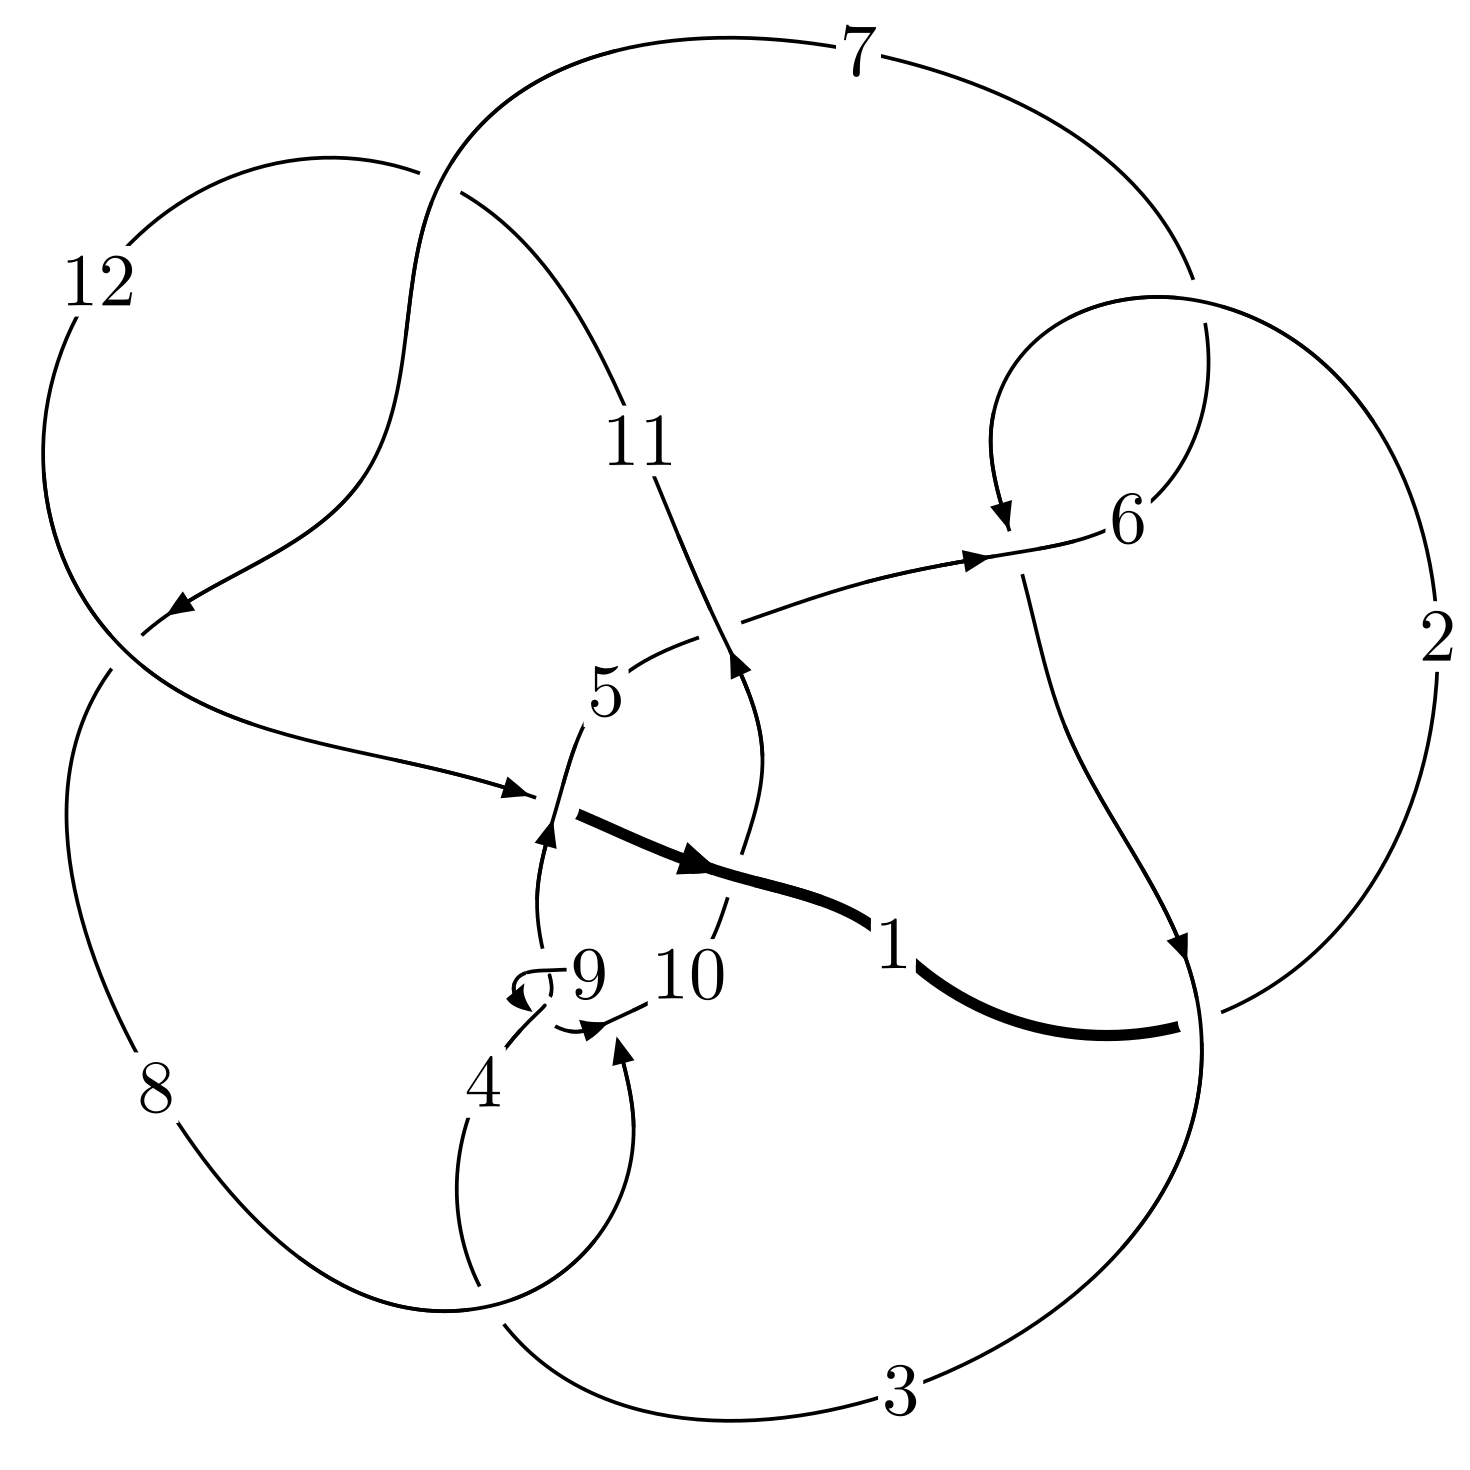
\includegraphics[width=112pt]{../../../GIT/diagram.site/Diagrams/png/1088_12a_0287.png}\\
\ \ \ A knot diagram\footnotemark}&
\allowdisplaybreaks
\textbf{Linearized knot diagam} \\
\cline{2-2}
 &
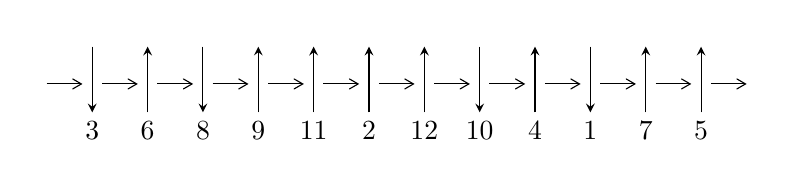
\begin{tikzpicture}[x=20pt, y=17pt]
	% nodes
	\node (C0) at (0, 0) {};
	\node (C1) at (1, 0) {};
	\node (C1U) at (1, +1) {};
	\node (C1D) at (1, -1) {3};

	\node (C2) at (2, 0) {};
	\node (C2U) at (2, +1) {};
	\node (C2D) at (2, -1) {6};

	\node (C3) at (3, 0) {};
	\node (C3U) at (3, +1) {};
	\node (C3D) at (3, -1) {8};

	\node (C4) at (4, 0) {};
	\node (C4U) at (4, +1) {};
	\node (C4D) at (4, -1) {9};

	\node (C5) at (5, 0) {};
	\node (C5U) at (5, +1) {};
	\node (C5D) at (5, -1) {11};

	\node (C6) at (6, 0) {};
	\node (C6U) at (6, +1) {};
	\node (C6D) at (6, -1) {2};

	\node (C7) at (7, 0) {};
	\node (C7U) at (7, +1) {};
	\node (C7D) at (7, -1) {12};

	\node (C8) at (8, 0) {};
	\node (C8U) at (8, +1) {};
	\node (C8D) at (8, -1) {10};

	\node (C9) at (9, 0) {};
	\node (C9U) at (9, +1) {};
	\node (C9D) at (9, -1) {4};

	\node (C10) at (10, 0) {};
	\node (C10U) at (10, +1) {};
	\node (C10D) at (10, -1) {1};

	\node (C11) at (11, 0) {};
	\node (C11U) at (11, +1) {};
	\node (C11D) at (11, -1) {7};

	\node (C12) at (12, 0) {};
	\node (C12U) at (12, +1) {};
	\node (C12D) at (12, -1) {5};
	\node (C13) at (13, 0) {};

	% arrows
	\draw[->,>={angle 60}]
	(C0) edge (C1) (C1) edge (C2) (C2) edge (C3) (C3) edge (C4) (C4) edge (C5) (C5) edge (C6) (C6) edge (C7) (C7) edge (C8) (C8) edge (C9) (C9) edge (C10) (C10) edge (C11) (C11) edge (C12) (C12) edge (C13) ;	\draw[->,>=stealth]
	(C1U) edge (C1D) (C2D) edge (C2U) (C3U) edge (C3D) (C4D) edge (C4U) (C5D) edge (C5U) (C6D) edge (C6U) (C7D) edge (C7U) (C8U) edge (C8D) (C9D) edge (C9U) (C10U) edge (C10D) (C11D) edge (C11U) (C12D) edge (C12U) ;
	\end{tikzpicture} \\
\hhline{~~} \\& 
\textbf{Solving Sequence} \\ \cline{2-2} 
 &
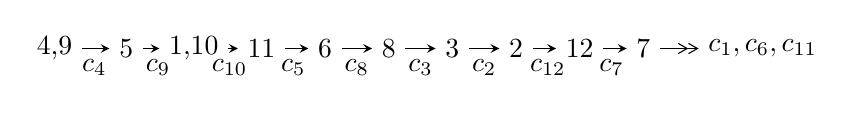
\begin{tikzpicture}[x=23pt, y=7pt]
	% node
	\node (A0) at (-1/8, 0) {4,9};
	\node (A1) at (1, 0) {5};
	\node (A2) at (33/16, 0) {1,10};
	\node (A3) at (25/8, 0) {11};
	\node (A4) at (33/8, 0) {6};
	\node (A5) at (41/8, 0) {8};
	\node (A6) at (49/8, 0) {3};
	\node (A7) at (57/8, 0) {2};
	\node (A8) at (65/8, 0) {12};
	\node (A9) at (73/8, 0) {7};
	\node (C1) at (1/2, -1) {$c_{4}$};
	\node (C2) at (3/2, -1) {$c_{9}$};
	\node (C3) at (21/8, -1) {$c_{10}$};
	\node (C4) at (29/8, -1) {$c_{5}$};
	\node (C5) at (37/8, -1) {$c_{8}$};
	\node (C6) at (45/8, -1) {$c_{3}$};
	\node (C7) at (53/8, -1) {$c_{2}$};
	\node (C8) at (61/8, -1) {$c_{12}$};
	\node (C9) at (69/8, -1) {$c_{7}$};
	\node (A10) at (11, 0) {$c_{1},c_{6},c_{11}$};

	% edge
	\draw[->,>=stealth]	
	(A0) edge (A1) (A1) edge (A2) (A2) edge (A3) (A3) edge (A4) (A4) edge (A5) (A5) edge (A6) (A6) edge (A7) (A7) edge (A8) (A8) edge (A9) ;
	\draw[->>,>={angle 60}]	
	(A9) edge (A10);
\end{tikzpicture} \\ 

\end{tabular} \\

\footnotetext{
The image of knot diagram is generated by the software ``\textbf{Draw programme}" developed by Andrew Bartholomew(\url{http://www.layer8.co.uk/maths/draw/index.htm\#Running-draw}), where we modified some parts for our purpose(\url{https://github.com/CATsTAILs/LinksPainter}).
}\phantom \\ \newline 
\centering \textbf{Ideals for irreducible components\footnotemark of $X_{\text{par}}$} 
 
\begin{align*}
I^u_{1}&=\langle 
-5.28450\times10^{165} u^{139}+9.50032\times10^{165} u^{138}+\cdots+4.17997\times10^{165} b+1.34496\times10^{167},\\
\phantom{I^u_{1}}&\phantom{= \langle  }-3.45422\times10^{167} u^{139}+5.01824\times10^{166} u^{138}+\cdots+9.19593\times10^{166} a+3.61218\times10^{168},\\
\phantom{I^u_{1}}&\phantom{= \langle  }u^{140}+u^{139}+\cdots+14 u+11\rangle \\
I^u_{2}&=\langle 
u^{27}+11 u^{25}+\cdots+b+10 u,\;5 u^{27}+37 u^{25}+\cdots+a+13 u,\;u^{28}+7 u^{26}+\cdots+5 u^2+1\rangle \\
I^u_{3}&=\langle 
u^2+b,\;u^2+a-1,\;u^9+u^7+u^5+u-1\rangle \\
\\
\end{align*}
\raggedright * 3 irreducible components of $\dim_{\mathbb{C}}=0$, with total 177 representations.\\
\footnotetext{All coefficients of polynomials are rational numbers. But the coefficients are sometimes approximated in decimal forms when there is not enough margin.}
\newpage
\renewcommand{\arraystretch}{1}
\centering \section*{I. $I^u_{1}= \langle -5.28\times10^{165} u^{139}+9.50\times10^{165} u^{138}+\cdots+4.18\times10^{165} b+1.34\times10^{167},\;-3.45\times10^{167} u^{139}+5.02\times10^{166} u^{138}+\cdots+9.20\times10^{166} a+3.61\times10^{168},\;u^{140}+u^{139}+\cdots+14 u+11 \rangle$}
\flushleft \textbf{(i) Arc colorings}\\
\begin{tabular}{m{7pt} m{180pt} m{7pt} m{180pt} }
\flushright $a_{4}=$&$\begin{pmatrix}1\\0\end{pmatrix}$ \\
\flushright $a_{9}=$&$\begin{pmatrix}0\\u\end{pmatrix}$ \\
\flushright $a_{5}=$&$\begin{pmatrix}1\\- u^2\end{pmatrix}$ \\
\flushright $a_{1}=$&$\begin{pmatrix}3.75625 u^{139}-0.545703 u^{138}+\cdots+18.3027 u-39.2802\\1.26424 u^{139}-2.27282 u^{138}+\cdots-5.05567 u-32.1762\end{pmatrix}$ \\
\flushright $a_{10}=$&$\begin{pmatrix}u\\u\end{pmatrix}$ \\
\flushright $a_{11}=$&$\begin{pmatrix}-4.21132 u^{139}-1.90514 u^{138}+\cdots-28.7256 u+13.4197\\-0.337816 u^{139}+0.850006 u^{138}+\cdots-35.4920 u+9.27420\end{pmatrix}$ \\
\flushright $a_{6}=$&$\begin{pmatrix}3.41851 u^{139}-0.916546 u^{138}+\cdots+18.8635 u-50.7061\\-0.955936 u^{139}-2.22549 u^{138}+\cdots+14.6427 u-34.2575\end{pmatrix}$ \\
\flushright $a_{8}=$&$\begin{pmatrix}u^3\\u^3+u\end{pmatrix}$ \\
\flushright $a_{3}=$&$\begin{pmatrix}- u^6- u^4+1\\- u^6-2 u^4- u^2\end{pmatrix}$ \\
\flushright $a_{2}=$&$\begin{pmatrix}3.41935 u^{139}-0.0188456 u^{138}+\cdots+15.9636 u-43.2660\\-0.152810 u^{139}-3.05181 u^{138}+\cdots-13.3247 u-36.1705\end{pmatrix}$ \\
\flushright $a_{12}=$&$\begin{pmatrix}2.90592 u^{139}-1.04471 u^{138}+\cdots+4.44981 u-54.4255\\0.423969 u^{139}-2.13116 u^{138}+\cdots-9.49081 u-28.3117\end{pmatrix}$ \\
\flushright $a_{7}=$&$\begin{pmatrix}-4.11706 u^{139}-1.14081 u^{138}+\cdots-23.6884 u+35.9336\\-2.17162 u^{139}-2.14855 u^{138}+\cdots-46.4276 u+7.90784\end{pmatrix}$\\&\end{tabular}
\flushleft \textbf{(ii) Obstruction class $= -1$}\\~\\
\flushleft \textbf{(iii) Cusp Shapes $= -2.40385 u^{139}+2.28727 u^{138}+\cdots-1.07060 u-7.80379$}\\~\\
\newpage\renewcommand{\arraystretch}{1}
\flushleft \textbf{(iv) u-Polynomials at the component}\newline \\
\begin{tabular}{m{50pt}|m{274pt}}
Crossings & \hspace{64pt}u-Polynomials at each crossing \\
\hline $$\begin{aligned}c_{1}\end{aligned}$$&$\begin{aligned}
&u^{140}+58 u^{139}+\cdots+876101 u+17161
\end{aligned}$\\
\hline $$\begin{aligned}c_{2},c_{6}\end{aligned}$$&$\begin{aligned}
&u^{140}-2 u^{139}+\cdots+17 u+131
\end{aligned}$\\
\hline $$\begin{aligned}c_{3}\end{aligned}$$&$\begin{aligned}
&u^{140}- u^{139}+\cdots-24244188 u+5702444
\end{aligned}$\\
\hline $$\begin{aligned}c_{4},c_{9}\end{aligned}$$&$\begin{aligned}
&u^{140}+u^{139}+\cdots+14 u+11
\end{aligned}$\\
\hline $$\begin{aligned}c_{5}\end{aligned}$$&$\begin{aligned}
&u^{140}+u^{139}+\cdots-143354 u+167897
\end{aligned}$\\
\hline $$\begin{aligned}c_{7},c_{11}\end{aligned}$$&$\begin{aligned}
&u^{140}+10 u^{139}+\cdots+49344 u+2992
\end{aligned}$\\
\hline $$\begin{aligned}c_{8}\end{aligned}$$&$\begin{aligned}
&u^{140}+71 u^{139}+\cdots+1322 u+121
\end{aligned}$\\
\hline $$\begin{aligned}c_{10}\end{aligned}$$&$\begin{aligned}
&u^{140}-23 u^{139}+\cdots+640 u+89
\end{aligned}$\\
\hline $$\begin{aligned}c_{12}\end{aligned}$$&$\begin{aligned}
&u^{140}- u^{139}+\cdots+26 u+1
\end{aligned}$\\
\hline
\end{tabular}\\~\\
\newpage\renewcommand{\arraystretch}{1}
\flushleft \textbf{(v) Riley Polynomials at the component}\newline \\
\begin{tabular}{m{50pt}|m{274pt}}
Crossings & \hspace{64pt}Riley Polynomials at each crossing \\
\hline $$\begin{aligned}c_{1}\end{aligned}$$&$\begin{aligned}
&y^{140}+62 y^{139}+\cdots-8770457803 y+294499921
\end{aligned}$\\
\hline $$\begin{aligned}c_{2},c_{6}\end{aligned}$$&$\begin{aligned}
&y^{140}+58 y^{139}+\cdots+876101 y+17161
\end{aligned}$\\
\hline $$\begin{aligned}c_{3}\end{aligned}$$&$\begin{aligned}
&y^{140}-57 y^{139}+\cdots-327195805998920 y+32517867573136
\end{aligned}$\\
\hline $$\begin{aligned}c_{4},c_{9}\end{aligned}$$&$\begin{aligned}
&y^{140}+71 y^{139}+\cdots+1322 y+121
\end{aligned}$\\
\hline $$\begin{aligned}c_{5}\end{aligned}$$&$\begin{aligned}
&y^{140}-39 y^{139}+\cdots-427794952430 y+28189402609
\end{aligned}$\\
\hline $$\begin{aligned}c_{7},c_{11}\end{aligned}$$&$\begin{aligned}
&y^{140}-102 y^{139}+\cdots-552000640 y+8952064
\end{aligned}$\\
\hline $$\begin{aligned}c_{8}\end{aligned}$$&$\begin{aligned}
&y^{140}+7 y^{139}+\cdots+781458 y+14641
\end{aligned}$\\
\hline $$\begin{aligned}c_{10}\end{aligned}$$&$\begin{aligned}
&y^{140}-13 y^{139}+\cdots-780196 y+7921
\end{aligned}$\\
\hline $$\begin{aligned}c_{12}\end{aligned}$$&$\begin{aligned}
&y^{140}-13 y^{139}+\cdots+104 y+1
\end{aligned}$\\
\hline
\end{tabular}\\~\\
\newpage\flushleft \textbf{(vi) Complex Volumes and Cusp Shapes}
$$\begin{array}{c|c|c}  
\text{Solutions to }I^u_{1}& \I (\text{vol} + \sqrt{-1}CS) & \text{Cusp shape}\\
 \hline 
\begin{aligned}
u &= \phantom{-}0.911969 + 0.414142 I \\
a &= -0.295171 + 0.791970 I \\
b &= \phantom{-}0.539256 + 0.590000 I\end{aligned}
 & \phantom{-}1.31840 - 4.43564 I & \phantom{-0.000000 } 0 \\ \hline\begin{aligned}
u &= \phantom{-}0.911969 - 0.414142 I \\
a &= -0.295171 - 0.791970 I \\
b &= \phantom{-}0.539256 - 0.590000 I\end{aligned}
 & \phantom{-}1.31840 + 4.43564 I & \phantom{-0.000000 } 0 \\ \hline\begin{aligned}
u &= -0.724107 + 0.706862 I \\
a &= \phantom{-}1.57131 - 0.24069 I \\
b &= \phantom{-}1.33717 + 0.90378 I\end{aligned}
 & \phantom{-}7.44163 - 5.54565 I & \phantom{-0.000000 } 0 \\ \hline\begin{aligned}
u &= -0.724107 - 0.706862 I \\
a &= \phantom{-}1.57131 + 0.24069 I \\
b &= \phantom{-}1.33717 - 0.90378 I\end{aligned}
 & \phantom{-}7.44163 + 5.54565 I & \phantom{-0.000000 } 0 \\ \hline\begin{aligned}
u &= \phantom{-}0.573448 + 0.872478 I \\
a &= -1.38716 + 0.30535 I \\
b &= -1.41475 + 1.27921 I\end{aligned}
 & \phantom{-}0.98342 + 4.84804 I & \phantom{-0.000000 } 0 \\ \hline\begin{aligned}
u &= \phantom{-}0.573448 - 0.872478 I \\
a &= -1.38716 - 0.30535 I \\
b &= -1.41475 - 1.27921 I\end{aligned}
 & \phantom{-}0.98342 - 4.84804 I & \phantom{-0.000000 } 0 \\ \hline\begin{aligned}
u &= -0.249323 + 0.915343 I \\
a &= \phantom{-}0.113498 + 0.814881 I \\
b &= -0.415139 - 0.488688 I\end{aligned}
 & -3.96870 - 1.13105 I & \phantom{-0.000000 } 0 \\ \hline\begin{aligned}
u &= -0.249323 - 0.915343 I \\
a &= \phantom{-}0.113498 - 0.814881 I \\
b &= -0.415139 + 0.488688 I\end{aligned}
 & -3.96870 + 1.13105 I & \phantom{-0.000000 } 0 \\ \hline\begin{aligned}
u &= -0.371737 + 0.986379 I \\
a &= \phantom{-}1.31279 + 1.63815 I \\
b &= -0.17991 + 2.38626 I\end{aligned}
 & \phantom{-}1.05783 + 3.25130 I & \phantom{-0.000000 } 0 \\ \hline\begin{aligned}
u &= -0.371737 - 0.986379 I \\
a &= \phantom{-}1.31279 - 1.63815 I \\
b &= -0.17991 - 2.38626 I\end{aligned}
 & \phantom{-}1.05783 - 3.25130 I & \phantom{-0.000000 } 0\\
 \hline 
 \end{array}$$\newpage$$\begin{array}{c|c|c}  
\text{Solutions to }I^u_{1}& \I (\text{vol} + \sqrt{-1}CS) & \text{Cusp shape}\\
 \hline 
\begin{aligned}
u &= \phantom{-}0.503794 + 0.799252 I \\
a &= -0.859487 + 0.896640 I \\
b &= -0.12251 + 1.61088 I\end{aligned}
 & \phantom{-}1.76715 + 2.73079 I & \phantom{-0.000000 } 0 \\ \hline\begin{aligned}
u &= \phantom{-}0.503794 - 0.799252 I \\
a &= -0.859487 - 0.896640 I \\
b &= -0.12251 - 1.61088 I\end{aligned}
 & \phantom{-}1.76715 - 2.73079 I & \phantom{-0.000000 } 0 \\ \hline\begin{aligned}
u &= \phantom{-}0.319065 + 0.887593 I \\
a &= -1.53683 + 0.81693 I \\
b &= -1.94899 + 1.51337 I\end{aligned}
 & \phantom{-}1.17088 + 5.15716 I & \phantom{-0.000000 } 0 \\ \hline\begin{aligned}
u &= \phantom{-}0.319065 - 0.887593 I \\
a &= -1.53683 - 0.81693 I \\
b &= -1.94899 - 1.51337 I\end{aligned}
 & \phantom{-}1.17088 - 5.15716 I & \phantom{-0.000000 } 0 \\ \hline\begin{aligned}
u &= \phantom{-}0.760627 + 0.745237 I \\
a &= -1.45122 - 0.27255 I \\
b &= -1.30533 + 0.94896 I\end{aligned}
 & \phantom{-}5.97477 + 11.24740 I & \phantom{-0.000000 } 0 \\ \hline\begin{aligned}
u &= \phantom{-}0.760627 - 0.745237 I \\
a &= -1.45122 + 0.27255 I \\
b &= -1.30533 - 0.94896 I\end{aligned}
 & \phantom{-}5.97477 - 11.24740 I & \phantom{-0.000000 } 0 \\ \hline\begin{aligned}
u &= \phantom{-}0.386677 + 0.999740 I \\
a &= -1.44116 + 1.04277 I \\
b &= -0.41987 + 2.11426 I\end{aligned}
 & \phantom{-}1.72635 + 2.31795 I & \phantom{-0.000000 } 0 \\ \hline\begin{aligned}
u &= \phantom{-}0.386677 - 0.999740 I \\
a &= -1.44116 - 1.04277 I \\
b &= -0.41987 - 2.11426 I\end{aligned}
 & \phantom{-}1.72635 - 2.31795 I & \phantom{-0.000000 } 0 \\ \hline\begin{aligned}
u &= -0.529092 + 0.760841 I \\
a &= -2.18860 + 0.27623 I \\
b &= -1.37970 - 1.09749 I\end{aligned}
 & \phantom{-}1.35663 - 6.65828 I & \phantom{-0.000000 } 0 \\ \hline\begin{aligned}
u &= -0.529092 - 0.760841 I \\
a &= -2.18860 - 0.27623 I \\
b &= -1.37970 + 1.09749 I\end{aligned}
 & \phantom{-}1.35663 + 6.65828 I & \phantom{-0.000000 } 0\\
 \hline 
 \end{array}$$\newpage$$\begin{array}{c|c|c}  
\text{Solutions to }I^u_{1}& \I (\text{vol} + \sqrt{-1}CS) & \text{Cusp shape}\\
 \hline 
\begin{aligned}
u &= \phantom{-}0.882048 + 0.278481 I \\
a &= \phantom{-}0.009019 + 0.462736 I \\
b &= \phantom{-}0.146813 + 0.345498 I\end{aligned}
 & \phantom{-}0.167945 - 0.191438 I & \phantom{-0.000000 } 0 \\ \hline\begin{aligned}
u &= \phantom{-}0.882048 - 0.278481 I \\
a &= \phantom{-}0.009019 - 0.462736 I \\
b &= \phantom{-}0.146813 - 0.345498 I\end{aligned}
 & \phantom{-}0.167945 + 0.191438 I & \phantom{-0.000000 } 0 \\ \hline\begin{aligned}
u &= -0.911020 + 0.149587 I \\
a &= -0.404056 + 0.037828 I \\
b &= \phantom{-}0.174739 + 0.028208 I\end{aligned}
 & -0.81281 + 3.32987 I & \phantom{-0.000000 } 0 \\ \hline\begin{aligned}
u &= -0.911020 - 0.149587 I \\
a &= -0.404056 - 0.037828 I \\
b &= \phantom{-}0.174739 - 0.028208 I\end{aligned}
 & -0.81281 - 3.32987 I & \phantom{-0.000000 } 0 \\ \hline\begin{aligned}
u &= -0.432089 + 0.996285 I \\
a &= -2.34096 - 0.75184 I \\
b &= -1.41076 - 1.40605 I\end{aligned}
 & \phantom{-}0.95739 - 6.37467 I & \phantom{-0.000000 } 0 \\ \hline\begin{aligned}
u &= -0.432089 - 0.996285 I \\
a &= -2.34096 + 0.75184 I \\
b &= -1.41076 + 1.40605 I\end{aligned}
 & \phantom{-}0.95739 + 6.37467 I & \phantom{-0.000000 } 0 \\ \hline\begin{aligned}
u &= -0.855066 + 0.311267 I \\
a &= -1.47002 - 0.74678 I \\
b &= \phantom{-}0.17531 - 1.42918 I\end{aligned}
 & \phantom{-}3.4637 + 14.2963 I & \phantom{-0.000000 } 0 \\ \hline\begin{aligned}
u &= -0.855066 - 0.311267 I \\
a &= -1.47002 + 0.74678 I \\
b &= \phantom{-}0.17531 + 1.42918 I\end{aligned}
 & \phantom{-}3.4637 - 14.2963 I & \phantom{-0.000000 } 0 \\ \hline\begin{aligned}
u &= \phantom{-}0.383480 + 1.044560 I \\
a &= \phantom{-}1.29468 - 2.09361 I \\
b &= \phantom{-}1.40886 - 2.17172 I\end{aligned}
 & \phantom{-}0.19673 - 2.64784 I & \phantom{-0.000000 } 0 \\ \hline\begin{aligned}
u &= \phantom{-}0.383480 - 1.044560 I \\
a &= \phantom{-}1.29468 + 2.09361 I \\
b &= \phantom{-}1.40886 + 2.17172 I\end{aligned}
 & \phantom{-}0.19673 + 2.64784 I & \phantom{-0.000000 } 0\\
 \hline 
 \end{array}$$\newpage$$\begin{array}{c|c|c}  
\text{Solutions to }I^u_{1}& \I (\text{vol} + \sqrt{-1}CS) & \text{Cusp shape}\\
 \hline 
\begin{aligned}
u &= \phantom{-}0.822294 + 0.316409 I \\
a &= \phantom{-}1.46564 - 0.72560 I \\
b &= -0.05027 - 1.48893 I\end{aligned}
 & \phantom{-}5.30338 - 8.23856 I & \phantom{-0.000000 } 0 \\ \hline\begin{aligned}
u &= \phantom{-}0.822294 - 0.316409 I \\
a &= \phantom{-}1.46564 + 0.72560 I \\
b &= -0.05027 + 1.48893 I\end{aligned}
 & \phantom{-}5.30338 + 8.23856 I & \phantom{-0.000000 } 0 \\ \hline\begin{aligned}
u &= -0.407338 + 1.046110 I \\
a &= \phantom{-}1.37012 + 0.73523 I \\
b &= \phantom{-}1.93075 + 1.96344 I\end{aligned}
 & \phantom{-}1.91948 - 1.55357 I & \phantom{-0.000000 } 0 \\ \hline\begin{aligned}
u &= -0.407338 - 1.046110 I \\
a &= \phantom{-}1.37012 - 0.73523 I \\
b &= \phantom{-}1.93075 - 1.96344 I\end{aligned}
 & \phantom{-}1.91948 + 1.55357 I & \phantom{-0.000000 } 0 \\ \hline\begin{aligned}
u &= -0.277132 + 1.091270 I \\
a &= \phantom{-}0.210019 + 0.713495 I \\
b &= -0.425588 + 0.144621 I\end{aligned}
 & -3.56177 - 0.25782 I & \phantom{-0.000000 } 0 \\ \hline\begin{aligned}
u &= -0.277132 - 1.091270 I \\
a &= \phantom{-}0.210019 - 0.713495 I \\
b &= -0.425588 - 0.144621 I\end{aligned}
 & -3.56177 + 0.25782 I & \phantom{-0.000000 } 0 \\ \hline\begin{aligned}
u &= \phantom{-}0.557324 + 0.670520 I \\
a &= \phantom{-}1.90723 + 0.19763 I \\
b &= \phantom{-}1.009950 - 0.920696 I\end{aligned}
 & \phantom{-}2.19061 + 1.51698 I & \phantom{-0.000000 } 0 \\ \hline\begin{aligned}
u &= \phantom{-}0.557324 - 0.670520 I \\
a &= \phantom{-}1.90723 - 0.19763 I \\
b &= \phantom{-}1.009950 + 0.920696 I\end{aligned}
 & \phantom{-}2.19061 - 1.51698 I & \phantom{-0.000000 } 0 \\ \hline\begin{aligned}
u &= -0.588752 + 0.639692 I \\
a &= \phantom{-}0.879389 + 0.930406 I \\
b &= -0.13286 + 1.46117 I\end{aligned}
 & \phantom{-}1.77091 + 2.37270 I & \phantom{-0.000000 } 0 \\ \hline\begin{aligned}
u &= -0.588752 - 0.639692 I \\
a &= \phantom{-}0.879389 - 0.930406 I \\
b &= -0.13286 - 1.46117 I\end{aligned}
 & \phantom{-}1.77091 - 2.37270 I & \phantom{-0.000000 } 0\\
 \hline 
 \end{array}$$\newpage$$\begin{array}{c|c|c}  
\text{Solutions to }I^u_{1}& \I (\text{vol} + \sqrt{-1}CS) & \text{Cusp shape}\\
 \hline 
\begin{aligned}
u &= -0.685835 + 0.900388 I \\
a &= -0.399211 - 1.303950 I \\
b &= \phantom{-}0.45329 - 1.43925 I\end{aligned}
 & \phantom{-}6.88187 + 0.21608 I & \phantom{-0.000000 } 0 \\ \hline\begin{aligned}
u &= -0.685835 - 0.900388 I \\
a &= -0.399211 + 1.303950 I \\
b &= \phantom{-}0.45329 + 1.43925 I\end{aligned}
 & \phantom{-}6.88187 - 0.21608 I & \phantom{-0.000000 } 0 \\ \hline\begin{aligned}
u &= -0.497345 + 1.026600 I \\
a &= -0.05339 - 2.30110 I \\
b &= \phantom{-}0.14269 - 2.52943 I\end{aligned}
 & \phantom{-}4.21178 - 2.96840 I & \phantom{-0.000000 } 0 \\ \hline\begin{aligned}
u &= -0.497345 - 1.026600 I \\
a &= -0.05339 + 2.30110 I \\
b &= \phantom{-}0.14269 + 2.52943 I\end{aligned}
 & \phantom{-}4.21178 + 2.96840 I & \phantom{-0.000000 } 0 \\ \hline\begin{aligned}
u &= \phantom{-}0.742425 + 0.885018 I \\
a &= \phantom{-}0.371900 - 1.170730 I \\
b &= -0.575239 - 1.275530 I\end{aligned}
 & \phantom{-}5.58093 - 5.64547 I & \phantom{-0.000000 } 0 \\ \hline\begin{aligned}
u &= \phantom{-}0.742425 - 0.885018 I \\
a &= \phantom{-}0.371900 + 1.170730 I \\
b &= -0.575239 + 1.275530 I\end{aligned}
 & \phantom{-}5.58093 + 5.64547 I & \phantom{-0.000000 } 0 \\ \hline\begin{aligned}
u &= -0.288711 + 1.120020 I \\
a &= \phantom{-}0.055580 + 0.507806 I \\
b &= -0.830418 - 0.229523 I\end{aligned}
 & -3.58932 + 0.00780 I & \phantom{-0.000000 } 0 \\ \hline\begin{aligned}
u &= -0.288711 - 1.120020 I \\
a &= \phantom{-}0.055580 - 0.507806 I \\
b &= -0.830418 + 0.229523 I\end{aligned}
 & -3.58932 - 0.00780 I & \phantom{-0.000000 } 0 \\ \hline\begin{aligned}
u &= \phantom{-}0.535179 + 1.051400 I \\
a &= -1.26686 + 0.76744 I \\
b &= -1.33178 + 2.30530 I\end{aligned}
 & \phantom{-}2.70191 + 0.79233 I & \phantom{-0.000000 } 0 \\ \hline\begin{aligned}
u &= \phantom{-}0.535179 - 1.051400 I \\
a &= -1.26686 - 0.76744 I \\
b &= -1.33178 - 2.30530 I\end{aligned}
 & \phantom{-}2.70191 - 0.79233 I & \phantom{-0.000000 } 0\\
 \hline 
 \end{array}$$\newpage$$\begin{array}{c|c|c}  
\text{Solutions to }I^u_{1}& \I (\text{vol} + \sqrt{-1}CS) & \text{Cusp shape}\\
 \hline 
\begin{aligned}
u &= \phantom{-}0.085516 + 1.180600 I \\
a &= -0.123421 + 0.432627 I \\
b &= -0.128542 - 0.518350 I\end{aligned}
 & -4.53995 - 1.81669 I & \phantom{-0.000000 } 0 \\ \hline\begin{aligned}
u &= \phantom{-}0.085516 - 1.180600 I \\
a &= -0.123421 - 0.432627 I \\
b &= -0.128542 + 0.518350 I\end{aligned}
 & -4.53995 + 1.81669 I & \phantom{-0.000000 } 0 \\ \hline\begin{aligned}
u &= -0.798315 + 0.158064 I \\
a &= -0.741241 + 0.157814 I \\
b &= -0.0818703 - 0.0112551 I\end{aligned}
 & -0.86862 + 3.34041 I & \phantom{-0.000000 } 0 \\ \hline\begin{aligned}
u &= -0.798315 - 0.158064 I \\
a &= -0.741241 - 0.157814 I \\
b &= -0.0818703 + 0.0112551 I\end{aligned}
 & -0.86862 - 3.34041 I & \phantom{-0.000000 } 0 \\ \hline\begin{aligned}
u &= \phantom{-}0.510897 + 1.071460 I \\
a &= \phantom{-}0.14755 - 1.82024 I \\
b &= -1.51281 - 1.36578 I\end{aligned}
 & \phantom{-}2.69466 + 4.26697 I & \phantom{-0.000000 } 0 \\ \hline\begin{aligned}
u &= \phantom{-}0.510897 - 1.071460 I \\
a &= \phantom{-}0.14755 + 1.82024 I \\
b &= -1.51281 + 1.36578 I\end{aligned}
 & \phantom{-}2.69466 - 4.26697 I & \phantom{-0.000000 } 0 \\ \hline\begin{aligned}
u &= -0.504019 + 1.077930 I \\
a &= \phantom{-}1.31667 + 0.76730 I \\
b &= \phantom{-}1.59642 + 2.35524 I\end{aligned}
 & \phantom{-}2.66785 - 5.26634 I & \phantom{-0.000000 } 0 \\ \hline\begin{aligned}
u &= -0.504019 - 1.077930 I \\
a &= \phantom{-}1.31667 - 0.76730 I \\
b &= \phantom{-}1.59642 - 2.35524 I\end{aligned}
 & \phantom{-}2.66785 + 5.26634 I & \phantom{-0.000000 } 0 \\ \hline\begin{aligned}
u &= -0.777543 + 0.223808 I \\
a &= -1.45938 - 0.71051 I \\
b &= -0.260728 - 1.189920 I\end{aligned}
 & -1.90870 + 5.88396 I & \phantom{-}4.00000 - 6.87965 I \\ \hline\begin{aligned}
u &= -0.777543 - 0.223808 I \\
a &= -1.45938 + 0.71051 I \\
b &= -0.260728 + 1.189920 I\end{aligned}
 & -1.90870 - 5.88396 I & \phantom{-}4.00000 + 6.87965 I\\
 \hline 
 \end{array}$$\newpage$$\begin{array}{c|c|c}  
\text{Solutions to }I^u_{1}& \I (\text{vol} + \sqrt{-1}CS) & \text{Cusp shape}\\
 \hline 
\begin{aligned}
u &= \phantom{-}0.379907 + 1.133040 I \\
a &= -0.392306 + 0.125578 I \\
b &= \phantom{-}0.359716 - 0.772154 I\end{aligned}
 & -7.48220 + 2.14063 I & \phantom{-0.000000 } 0 \\ \hline\begin{aligned}
u &= \phantom{-}0.379907 - 1.133040 I \\
a &= -0.392306 - 0.125578 I \\
b &= \phantom{-}0.359716 + 0.772154 I\end{aligned}
 & -7.48220 - 2.14063 I & \phantom{-0.000000 } 0 \\ \hline\begin{aligned}
u &= \phantom{-}0.764176 + 0.247294 I \\
a &= -1.78922 + 0.32789 I \\
b &= \phantom{-}0.212648 + 1.258030 I\end{aligned}
 & -0.93479 - 7.87402 I & \phantom{-}4.00000 + 7.57769 I \\ \hline\begin{aligned}
u &= \phantom{-}0.764176 - 0.247294 I \\
a &= -1.78922 - 0.32789 I \\
b &= \phantom{-}0.212648 - 1.258030 I\end{aligned}
 & -0.93479 + 7.87402 I & \phantom{-}4.00000 - 7.57769 I \\ \hline\begin{aligned}
u &= -0.530941 + 1.073870 I \\
a &= -0.59649 - 1.90781 I \\
b &= \phantom{-}1.22556 - 1.92500 I\end{aligned}
 & \phantom{-}2.35475 - 9.76727 I & \phantom{-0.000000 } 0 \\ \hline\begin{aligned}
u &= -0.530941 - 1.073870 I \\
a &= -0.59649 + 1.90781 I \\
b &= \phantom{-}1.22556 + 1.92500 I\end{aligned}
 & \phantom{-}2.35475 + 9.76727 I & \phantom{-0.000000 } 0 \\ \hline\begin{aligned}
u &= \phantom{-}0.511201 + 1.085870 I \\
a &= -0.81134 - 1.71392 I \\
b &= -0.84329 - 2.20566 I\end{aligned}
 & \phantom{-}1.15469 + 9.56512 I & \phantom{-0.000000 } 0 \\ \hline\begin{aligned}
u &= \phantom{-}0.511201 - 1.085870 I \\
a &= -0.81134 + 1.71392 I \\
b &= -0.84329 + 2.20566 I\end{aligned}
 & \phantom{-}1.15469 - 9.56512 I & \phantom{-0.000000 } 0 \\ \hline\begin{aligned}
u &= -0.715536 + 0.348808 I \\
a &= \phantom{-}0.947491 + 0.152160 I \\
b &= \phantom{-}0.076459 + 1.040320 I\end{aligned}
 & \phantom{-}0.59136 + 2.31044 I & \phantom{-}4.00000 - 5.49298 I \\ \hline\begin{aligned}
u &= -0.715536 - 0.348808 I \\
a &= \phantom{-}0.947491 - 0.152160 I \\
b &= \phantom{-}0.076459 - 1.040320 I\end{aligned}
 & \phantom{-}0.59136 - 2.31044 I & \phantom{-}4.00000 + 5.49298 I\\
 \hline 
 \end{array}$$\newpage$$\begin{array}{c|c|c}  
\text{Solutions to }I^u_{1}& \I (\text{vol} + \sqrt{-1}CS) & \text{Cusp shape}\\
 \hline 
\begin{aligned}
u &= \phantom{-}0.300124 + 1.170360 I \\
a &= \phantom{-}0.060639 + 0.271340 I \\
b &= \phantom{-}1.053180 - 0.615704 I\end{aligned}
 & -5.22041 - 4.56927 I & \phantom{-0.000000 } 0 \\ \hline\begin{aligned}
u &= \phantom{-}0.300124 - 1.170360 I \\
a &= \phantom{-}0.060639 - 0.271340 I \\
b &= \phantom{-}1.053180 + 0.615704 I\end{aligned}
 & -5.22041 + 4.56927 I & \phantom{-0.000000 } 0 \\ \hline\begin{aligned}
u &= \phantom{-}0.222165 + 1.188980 I \\
a &= \phantom{-}0.569913 - 0.345685 I \\
b &= -0.323401 + 0.381331 I\end{aligned}
 & \phantom{-}0.41796 - 5.15841 I & \phantom{-0.000000 } 0 \\ \hline\begin{aligned}
u &= \phantom{-}0.222165 - 1.188980 I \\
a &= \phantom{-}0.569913 + 0.345685 I \\
b &= -0.323401 - 0.381331 I\end{aligned}
 & \phantom{-}0.41796 + 5.15841 I & \phantom{-0.000000 } 0 \\ \hline\begin{aligned}
u &= \phantom{-}0.503060 + 1.102730 I \\
a &= -0.705803 + 0.647032 I \\
b &= -0.59454 + 1.28486 I\end{aligned}
 & -1.09806 + 3.76347 I & \phantom{-0.000000 } 0 \\ \hline\begin{aligned}
u &= \phantom{-}0.503060 - 1.102730 I \\
a &= -0.705803 - 0.647032 I \\
b &= -0.59454 - 1.28486 I\end{aligned}
 & -1.09806 - 3.76347 I & \phantom{-0.000000 } 0 \\ \hline\begin{aligned}
u &= \phantom{-}0.525428 + 1.094590 I \\
a &= -2.09927 + 1.37574 I \\
b &= -1.36521 + 1.80930 I\end{aligned}
 & \phantom{-}2.95162 + 7.00188 I & \phantom{-0.000000 } 0 \\ \hline\begin{aligned}
u &= \phantom{-}0.525428 - 1.094590 I \\
a &= -2.09927 - 1.37574 I \\
b &= -1.36521 - 1.80930 I\end{aligned}
 & \phantom{-}2.95162 - 7.00188 I & \phantom{-0.000000 } 0 \\ \hline\begin{aligned}
u &= \phantom{-}0.390175 + 1.152860 I \\
a &= -0.237640 - 0.174763 I \\
b &= -0.434998 + 0.526964 I\end{aligned}
 & -1.73181 + 3.89697 I & \phantom{-0.000000 } 0 \\ \hline\begin{aligned}
u &= \phantom{-}0.390175 - 1.152860 I \\
a &= -0.237640 + 0.174763 I \\
b &= -0.434998 - 0.526964 I\end{aligned}
 & -1.73181 - 3.89697 I & \phantom{-0.000000 } 0\\
 \hline 
 \end{array}$$\newpage$$\begin{array}{c|c|c}  
\text{Solutions to }I^u_{1}& \I (\text{vol} + \sqrt{-1}CS) & \text{Cusp shape}\\
 \hline 
\begin{aligned}
u &= -0.725049 + 0.286531 I \\
a &= \phantom{-}1.59501 + 0.27107 I \\
b &= -0.073027 + 1.258600 I\end{aligned}
 & \phantom{-}0.56147 + 2.93715 I & \phantom{-}6.93912 - 3.36871 I \\ \hline\begin{aligned}
u &= -0.725049 - 0.286531 I \\
a &= \phantom{-}1.59501 - 0.27107 I \\
b &= -0.073027 - 1.258600 I\end{aligned}
 & \phantom{-}0.56147 - 2.93715 I & \phantom{-}6.93912 + 3.36871 I \\ \hline\begin{aligned}
u &= \phantom{-}0.256246 + 1.194190 I \\
a &= -0.403224 + 0.526139 I \\
b &= -0.428589 + 0.014810 I\end{aligned}
 & -4.69523 + 3.15950 I & \phantom{-0.000000 } 0 \\ \hline\begin{aligned}
u &= \phantom{-}0.256246 - 1.194190 I \\
a &= -0.403224 - 0.526139 I \\
b &= -0.428589 - 0.014810 I\end{aligned}
 & -4.69523 - 3.15950 I & \phantom{-0.000000 } 0 \\ \hline\begin{aligned}
u &= -0.309365 + 1.185560 I \\
a &= -0.860502 + 0.079393 I \\
b &= -0.199008 + 0.683391 I\end{aligned}
 & -6.20028 + 2.41913 I & \phantom{-0.000000 } 0 \\ \hline\begin{aligned}
u &= -0.309365 - 1.185560 I \\
a &= -0.860502 - 0.079393 I \\
b &= -0.199008 - 0.683391 I\end{aligned}
 & -6.20028 - 2.41913 I & \phantom{-0.000000 } 0 \\ \hline\begin{aligned}
u &= \phantom{-}0.493769 + 1.131300 I \\
a &= \phantom{-}1.84984 - 1.07514 I \\
b &= \phantom{-}1.68788 - 2.15259 I\end{aligned}
 & -6.69268 + 5.68760 I & \phantom{-0.000000 } 0 \\ \hline\begin{aligned}
u &= \phantom{-}0.493769 - 1.131300 I \\
a &= \phantom{-}1.84984 + 1.07514 I \\
b &= \phantom{-}1.68788 + 2.15259 I\end{aligned}
 & -6.69268 - 5.68760 I & \phantom{-0.000000 } 0 \\ \hline\begin{aligned}
u &= -0.412124 + 1.164170 I \\
a &= \phantom{-}0.658848 + 0.730608 I \\
b &= \phantom{-}0.647271 + 0.996129 I\end{aligned}
 & -4.64683 - 0.60445 I & \phantom{-0.000000 } 0 \\ \hline\begin{aligned}
u &= -0.412124 - 1.164170 I \\
a &= \phantom{-}0.658848 - 0.730608 I \\
b &= \phantom{-}0.647271 - 0.996129 I\end{aligned}
 & -4.64683 + 0.60445 I & \phantom{-0.000000 } 0\\
 \hline 
 \end{array}$$\newpage$$\begin{array}{c|c|c}  
\text{Solutions to }I^u_{1}& \I (\text{vol} + \sqrt{-1}CS) & \text{Cusp shape}\\
 \hline 
\begin{aligned}
u &= -0.268998 + 0.715960 I \\
a &= -1.06054 - 2.24870 I \\
b &= -0.680161 - 1.093680 I\end{aligned}
 & \phantom{-}3.35259 - 1.39528 I & \phantom{-}1.67927 + 4.08016 I \\ \hline\begin{aligned}
u &= -0.268998 - 0.715960 I \\
a &= -1.06054 + 2.24870 I \\
b &= -0.680161 + 1.093680 I\end{aligned}
 & \phantom{-}3.35259 + 1.39528 I & \phantom{-}1.67927 - 4.08016 I \\ \hline\begin{aligned}
u &= -0.309936 + 0.693725 I \\
a &= -1.48957 + 1.16494 I \\
b &= -1.51730 + 0.18423 I\end{aligned}
 & -2.72477 - 1.41570 I & -0.24846 + 4.76390 I \\ \hline\begin{aligned}
u &= -0.309936 - 0.693725 I \\
a &= -1.48957 - 1.16494 I \\
b &= -1.51730 - 0.18423 I\end{aligned}
 & -2.72477 + 1.41570 I & -0.24846 - 4.76390 I \\ \hline\begin{aligned}
u &= -0.556829 + 1.112940 I \\
a &= -1.33823 - 0.91168 I \\
b &= -0.68459 - 1.72487 I\end{aligned}
 & -1.64506 - 7.18301 I & \phantom{-0.000000 } 0 \\ \hline\begin{aligned}
u &= -0.556829 - 1.112940 I \\
a &= -1.33823 + 0.91168 I \\
b &= -0.68459 + 1.72487 I\end{aligned}
 & -1.64506 + 7.18301 I & \phantom{-0.000000 } 0 \\ \hline\begin{aligned}
u &= -0.217648 + 1.225930 I \\
a &= -0.420472 - 0.246603 I \\
b &= \phantom{-}0.455392 + 0.573187 I\end{aligned}
 & -1.61265 + 11.02410 I & \phantom{-0.000000 } 0 \\ \hline\begin{aligned}
u &= -0.217648 - 1.225930 I \\
a &= -0.420472 + 0.246603 I \\
b &= \phantom{-}0.455392 - 0.573187 I\end{aligned}
 & -1.61265 - 11.02410 I & \phantom{-0.000000 } 0 \\ \hline\begin{aligned}
u &= \phantom{-}0.607376 + 0.445106 I \\
a &= \phantom{-}2.40457 - 0.89073 I \\
b &= \phantom{-}0.100803 - 0.915692 I\end{aligned}
 & \phantom{-}4.46559 + 3.74657 I & \phantom{-}10.94549 - 5.79337 I \\ \hline\begin{aligned}
u &= \phantom{-}0.607376 - 0.445106 I \\
a &= \phantom{-}2.40457 + 0.89073 I \\
b &= \phantom{-}0.100803 + 0.915692 I\end{aligned}
 & \phantom{-}4.46559 - 3.74657 I & \phantom{-}10.94549 + 5.79337 I\\
 \hline 
 \end{array}$$\newpage$$\begin{array}{c|c|c}  
\text{Solutions to }I^u_{1}& \I (\text{vol} + \sqrt{-1}CS) & \text{Cusp shape}\\
 \hline 
\begin{aligned}
u &= -0.542497 + 1.128160 I \\
a &= -1.71190 - 1.08526 I \\
b &= -1.18635 - 2.35380 I\end{aligned}
 & -1.87982 - 7.74973 I & \phantom{-0.000000 } 0 \\ \hline\begin{aligned}
u &= -0.542497 - 1.128160 I \\
a &= -1.71190 + 1.08526 I \\
b &= -1.18635 + 2.35380 I\end{aligned}
 & -1.87982 + 7.74973 I & \phantom{-0.000000 } 0 \\ \hline\begin{aligned}
u &= -0.271336 + 1.223150 I \\
a &= \phantom{-}0.158492 + 0.175972 I \\
b &= \phantom{-}0.197295 + 0.823123 I\end{aligned}
 & -5.55443 - 0.46075 I & \phantom{-0.000000 } 0 \\ \hline\begin{aligned}
u &= -0.271336 - 1.223150 I \\
a &= \phantom{-}0.158492 - 0.175972 I \\
b &= \phantom{-}0.197295 - 0.823123 I\end{aligned}
 & -5.55443 + 0.46075 I & \phantom{-0.000000 } 0 \\ \hline\begin{aligned}
u &= -0.536975 + 0.504589 I \\
a &= \phantom{-}2.29279 - 0.29116 I \\
b &= \phantom{-}1.80332 + 0.27481 I\end{aligned}
 & \phantom{-}5.74913 - 1.25065 I & \phantom{-}17.0911 + 2.4895 I \\ \hline\begin{aligned}
u &= -0.536975 - 0.504589 I \\
a &= \phantom{-}2.29279 + 0.29116 I \\
b &= \phantom{-}1.80332 - 0.27481 I\end{aligned}
 & \phantom{-}5.74913 + 1.25065 I & \phantom{-}17.0911 - 2.4895 I \\ \hline\begin{aligned}
u &= -0.616872 + 0.399769 I \\
a &= \phantom{-}1.11263 - 1.45968 I \\
b &= \phantom{-}1.08954 + 1.16118 I\end{aligned}
 & \phantom{-}4.31207 + 5.22253 I & \phantom{-}11.41114 - 7.60039 I \\ \hline\begin{aligned}
u &= -0.616872 - 0.399769 I \\
a &= \phantom{-}1.11263 + 1.45968 I \\
b &= \phantom{-}1.08954 - 1.16118 I\end{aligned}
 & \phantom{-}4.31207 - 5.22253 I & \phantom{-}11.41114 + 7.60039 I \\ \hline\begin{aligned}
u &= \phantom{-}0.542135 + 1.149850 I \\
a &= \phantom{-}1.78469 - 1.12003 I \\
b &= \phantom{-}1.39724 - 2.59801 I\end{aligned}
 & -3.56785 + 12.76600 I & \phantom{-0.000000 } 0 \\ \hline\begin{aligned}
u &= \phantom{-}0.542135 - 1.149850 I \\
a &= \phantom{-}1.78469 + 1.12003 I \\
b &= \phantom{-}1.39724 + 2.59801 I\end{aligned}
 & -3.56785 - 12.76600 I & \phantom{-0.000000 } 0\\
 \hline 
 \end{array}$$\newpage$$\begin{array}{c|c|c}  
\text{Solutions to }I^u_{1}& \I (\text{vol} + \sqrt{-1}CS) & \text{Cusp shape}\\
 \hline 
\begin{aligned}
u &= -0.537064 + 1.158640 I \\
a &= \phantom{-}1.63348 + 1.41062 I \\
b &= \phantom{-}1.40218 + 2.24229 I\end{aligned}
 & -4.64179 - 10.77630 I & \phantom{-0.000000 } 0 \\ \hline\begin{aligned}
u &= -0.537064 - 1.158640 I \\
a &= \phantom{-}1.63348 - 1.41062 I \\
b &= \phantom{-}1.40218 - 2.24229 I\end{aligned}
 & -4.64179 + 10.77630 I & \phantom{-0.000000 } 0 \\ \hline\begin{aligned}
u &= -0.629792 + 1.120880 I \\
a &= -1.384600 - 0.218094 I \\
b &= -1.35353 - 1.13882 I\end{aligned}
 & -0.38936 - 5.55432 I & \phantom{-0.000000 } 0 \\ \hline\begin{aligned}
u &= -0.629792 - 1.120880 I \\
a &= -1.384600 + 0.218094 I \\
b &= -1.35353 + 1.13882 I\end{aligned}
 & -0.38936 + 5.55432 I & \phantom{-0.000000 } 0 \\ \hline\begin{aligned}
u &= \phantom{-}0.628629 + 0.334137 I \\
a &= \phantom{-}1.22200 - 0.78546 I \\
b &= \phantom{-}0.49265 - 1.81699 I\end{aligned}
 & \phantom{-}5.13183 - 2.46029 I & \phantom{-}14.5121 + 3.1935 I \\ \hline\begin{aligned}
u &= \phantom{-}0.628629 - 0.334137 I \\
a &= \phantom{-}1.22200 + 0.78546 I \\
b &= \phantom{-}0.49265 + 1.81699 I\end{aligned}
 & \phantom{-}5.13183 + 2.46029 I & \phantom{-}14.5121 - 3.1935 I \\ \hline\begin{aligned}
u &= \phantom{-}0.579520 + 1.151040 I \\
a &= -1.84127 + 1.20626 I \\
b &= -1.42150 + 2.37650 I\end{aligned}
 & \phantom{-}2.81809 + 13.44720 I & \phantom{-0.000000 } 0 \\ \hline\begin{aligned}
u &= \phantom{-}0.579520 - 1.151040 I \\
a &= -1.84127 - 1.20626 I \\
b &= -1.42150 - 2.37650 I\end{aligned}
 & \phantom{-}2.81809 - 13.44720 I & \phantom{-0.000000 } 0 \\ \hline\begin{aligned}
u &= -0.539679 + 1.174260 I \\
a &= \phantom{-}0.519756 + 0.565749 I \\
b &= \phantom{-}0.568295 + 1.209960 I\end{aligned}
 & -3.78985 - 8.29502 I & \phantom{-0.000000 } 0 \\ \hline\begin{aligned}
u &= -0.539679 - 1.174260 I \\
a &= \phantom{-}0.519756 - 0.565749 I \\
b &= \phantom{-}0.568295 - 1.209960 I\end{aligned}
 & -3.78985 + 8.29502 I & \phantom{-0.000000 } 0\\
 \hline 
 \end{array}$$\newpage$$\begin{array}{c|c|c}  
\text{Solutions to }I^u_{1}& \I (\text{vol} + \sqrt{-1}CS) & \text{Cusp shape}\\
 \hline 
\begin{aligned}
u &= -0.588027 + 1.163950 I \\
a &= \phantom{-}1.82276 + 1.12851 I \\
b &= \phantom{-}1.50080 + 2.40647 I\end{aligned}
 & \phantom{-}0.9078 - 19.6213 I & \phantom{-0.000000 } 0 \\ \hline\begin{aligned}
u &= -0.588027 - 1.163950 I \\
a &= \phantom{-}1.82276 - 1.12851 I \\
b &= \phantom{-}1.50080 - 2.40647 I\end{aligned}
 & \phantom{-}0.9078 + 19.6213 I & \phantom{-0.000000 } 0 \\ \hline\begin{aligned}
u &= \phantom{-}0.557247 + 1.181640 I \\
a &= \phantom{-}0.792973 - 0.315005 I \\
b &= \phantom{-}0.704654 - 0.506911 I\end{aligned}
 & -2.62882 + 5.45005 I & \phantom{-0.000000 } 0 \\ \hline\begin{aligned}
u &= \phantom{-}0.557247 - 1.181640 I \\
a &= \phantom{-}0.792973 + 0.315005 I \\
b &= \phantom{-}0.704654 + 0.506911 I\end{aligned}
 & -2.62882 - 5.45005 I & \phantom{-0.000000 } 0 \\ \hline\begin{aligned}
u &= -0.435170 + 1.232080 I \\
a &= -0.1230310 - 0.0430721 I \\
b &= -0.042932 + 0.484585 I\end{aligned}
 & -4.41309 - 8.15300 I & \phantom{-0.000000 } 0 \\ \hline\begin{aligned}
u &= -0.435170 - 1.232080 I \\
a &= -0.1230310 + 0.0430721 I \\
b &= -0.042932 - 0.484585 I\end{aligned}
 & -4.41309 + 8.15300 I & \phantom{-0.000000 } 0 \\ \hline\begin{aligned}
u &= \phantom{-}0.567332 + 0.394477 I \\
a &= \phantom{-}1.019630 + 0.074384 I \\
b &= \phantom{-}0.363102 - 0.269838 I\end{aligned}
 & \phantom{-}1.049830 + 0.546340 I & \phantom{-}8.89907 - 4.13660 I \\ \hline\begin{aligned}
u &= \phantom{-}0.567332 - 0.394477 I \\
a &= \phantom{-}1.019630 - 0.074384 I \\
b &= \phantom{-}0.363102 + 0.269838 I\end{aligned}
 & \phantom{-}1.049830 - 0.546340 I & \phantom{-}8.89907 + 4.13660 I \\ \hline\begin{aligned}
u &= \phantom{-}0.631252 + 1.156750 I \\
a &= \phantom{-}1.223300 - 0.130066 I \\
b &= \phantom{-}1.36556 - 0.88130 I\end{aligned}
 & -0.97757 + 10.10480 I & \phantom{-0.000000 } 0 \\ \hline\begin{aligned}
u &= \phantom{-}0.631252 - 1.156750 I \\
a &= \phantom{-}1.223300 + 0.130066 I \\
b &= \phantom{-}1.36556 + 0.88130 I\end{aligned}
 & -0.97757 - 10.10480 I & \phantom{-0.000000 } 0\\
 \hline 
 \end{array}$$\newpage$$\begin{array}{c|c|c}  
\text{Solutions to }I^u_{1}& \I (\text{vol} + \sqrt{-1}CS) & \text{Cusp shape}\\
 \hline 
\begin{aligned}
u &= -0.524327 + 0.417163 I \\
a &= -0.767776 - 0.494553 I \\
b &= -0.45482 - 1.90743 I\end{aligned}
 & \phantom{-}3.51278 - 4.24004 I & \phantom{-}10.95131 + 5.69177 I \\ \hline\begin{aligned}
u &= -0.524327 - 0.417163 I \\
a &= -0.767776 + 0.494553 I \\
b &= -0.45482 + 1.90743 I\end{aligned}
 & \phantom{-}3.51278 + 4.24004 I & \phantom{-}10.95131 - 5.69177 I \\ \hline\begin{aligned}
u &= \phantom{-}0.550711 + 0.376242 I \\
a &= -0.60192 - 1.85435 I \\
b &= -1.25214 + 0.79998 I\end{aligned}
 & \phantom{-}4.68590 + 0.06128 I & \phantom{-}11.69405 + 1.52199 I \\ \hline\begin{aligned}
u &= \phantom{-}0.550711 - 0.376242 I \\
a &= -0.60192 + 1.85435 I \\
b &= -1.25214 - 0.79998 I\end{aligned}
 & \phantom{-}4.68590 - 0.06128 I & \phantom{-}11.69405 - 1.52199 I \\ \hline\begin{aligned}
u &= \phantom{-}0.644120 + 0.158741 I \\
a &= -1.73023 + 0.65345 I \\
b &= \phantom{-}0.062149 + 1.058440 I\end{aligned}
 & -3.99564 - 1.31752 I & -0.467328 + 0.682592 I \\ \hline\begin{aligned}
u &= \phantom{-}0.644120 - 0.158741 I \\
a &= -1.73023 - 0.65345 I \\
b &= \phantom{-}0.062149 - 1.058440 I\end{aligned}
 & -3.99564 + 1.31752 I & -0.467328 - 0.682592 I \\ \hline\begin{aligned}
u &= \phantom{-}0.566261 + 0.341356 I \\
a &= -2.17889 - 0.76525 I \\
b &= -1.276800 - 0.452358 I\end{aligned}
 & \phantom{-}3.27891 - 5.20337 I & \phantom{-}9.05791 + 8.92202 I \\ \hline\begin{aligned}
u &= \phantom{-}0.566261 - 0.341356 I \\
a &= -2.17889 + 0.76525 I \\
b &= -1.276800 + 0.452358 I\end{aligned}
 & \phantom{-}3.27891 + 5.20337 I & \phantom{-}9.05791 - 8.92202 I \\ \hline\begin{aligned}
u &= -0.529988 + 0.369897 I \\
a &= -2.77730 - 1.24477 I \\
b &= -0.121672 - 0.729596 I\end{aligned}
 & \phantom{-}4.70950 + 1.00343 I & \phantom{-}11.45787 - 2.33178 I \\ \hline\begin{aligned}
u &= -0.529988 - 0.369897 I \\
a &= -2.77730 + 1.24477 I \\
b &= -0.121672 + 0.729596 I\end{aligned}
 & \phantom{-}4.70950 - 1.00343 I & \phantom{-}11.45787 + 2.33178 I\\
 \hline 
 \end{array}$$\newpage\newpage\renewcommand{\arraystretch}{1}
\centering \section*{II. $I^u_{2}= \langle u^{27}+11 u^{25}+\cdots+b+10 u,\;5 u^{27}+37 u^{25}+\cdots+a+13 u,\;u^{28}+7 u^{26}+\cdots+5 u^2+1 \rangle$}
\flushleft \textbf{(i) Arc colorings}\\
\begin{tabular}{m{7pt} m{180pt} m{7pt} m{180pt} }
\flushright $a_{4}=$&$\begin{pmatrix}1\\0\end{pmatrix}$ \\
\flushright $a_{9}=$&$\begin{pmatrix}0\\u\end{pmatrix}$ \\
\flushright $a_{5}=$&$\begin{pmatrix}1\\- u^2\end{pmatrix}$ \\
\flushright $a_{1}=$&$\begin{pmatrix}-5 u^{27}-37 u^{25}+\cdots-54 u^3-13 u\\- u^{27}-11 u^{25}+\cdots-36 u^3-10 u\end{pmatrix}$ \\
\flushright $a_{10}=$&$\begin{pmatrix}u\\u\end{pmatrix}$ \\
\flushright $a_{11}=$&$\begin{pmatrix}4 u^{27}+5 u^{26}+\cdots+u+3\\2 u^{27}+3 u^{26}+\cdots+5 u+5\end{pmatrix}$ \\
\flushright $a_{6}=$&$\begin{pmatrix}6 u^{27}- u^{26}+\cdots+5 u-7\\4 u^{27}+u^{26}+\cdots+6 u-4\end{pmatrix}$ \\
\flushright $a_{8}=$&$\begin{pmatrix}u^3\\u^3+u\end{pmatrix}$ \\
\flushright $a_{3}=$&$\begin{pmatrix}- u^6- u^4+1\\- u^6-2 u^4- u^2\end{pmatrix}$ \\
\flushright $a_{2}=$&$\begin{pmatrix}-2 u^{27}-16 u^{25}+\cdots-24 u^3-6 u\\u^{27}+3 u^{25}+\cdots-19 u^3-6 u\end{pmatrix}$ \\
\flushright $a_{12}=$&$\begin{pmatrix}-2 u^{27}-17 u^{25}+\cdots-30 u^3-8 u\\-4 u^{25}-25 u^{23}+\cdots-26 u^3-7 u\end{pmatrix}$ \\
\flushright $a_{7}=$&$\begin{pmatrix}7 u^{27}+44 u^{25}+\cdots+8 u+1\\7 u^{27}- u^{26}+\cdots- u^2+12 u\end{pmatrix}$\\&\end{tabular}
\flushleft \textbf{(ii) Obstruction class $= 1$}\\~\\
\flushleft \textbf{(iii) Cusp Shapes $= 8 u^{27}-8 u^{26}+56 u^{25}-48 u^{24}+199 u^{23}-160 u^{22}+448 u^{21}-345 u^{20}+699 u^{19}-548 u^{18}+809 u^{17}-678 u^{16}+768 u^{15}-716 u^{14}+718 u^{13}-661 u^{12}+695 u^{11}-535 u^{10}+617 u^9-351 u^8+417 u^7-196 u^6+218 u^5-92 u^4+77 u^3-40 u^2+21 u$}\\~\\
\newpage\renewcommand{\arraystretch}{1}
\flushleft \textbf{(iv) u-Polynomials at the component}\newline \\
\begin{tabular}{m{50pt}|m{274pt}}
Crossings & \hspace{64pt}u-Polynomials at each crossing \\
\hline $$\begin{aligned}c_{1}\end{aligned}$$&$\begin{aligned}
&u^{28}-13 u^{27}+\cdots-13 u+1
\end{aligned}$\\
\hline $$\begin{aligned}c_{2}\end{aligned}$$&$\begin{aligned}
&u^{28}- u^{27}+\cdots- u+1
\end{aligned}$\\
\hline $$\begin{aligned}c_{3}\end{aligned}$$&$\begin{aligned}
&u^{28}-5 u^{26}+\cdots-3 u+2
\end{aligned}$\\
\hline $$\begin{aligned}c_{4}\end{aligned}$$&$\begin{aligned}
&u^{28}+7 u^{26}+\cdots+5 u^2+1
\end{aligned}$\\
\hline $$\begin{aligned}c_{5}\end{aligned}$$&$\begin{aligned}
&u^{28}+2 u^{26}+\cdots- u^2+1
\end{aligned}$\\
\hline $$\begin{aligned}c_{6}\end{aligned}$$&$\begin{aligned}
&u^{28}+u^{27}+\cdots+u+1
\end{aligned}$\\
\hline $$\begin{aligned}c_{7}\end{aligned}$$&$\begin{aligned}
&u^{28}-2 u^{27}+\cdots-9 u+2
\end{aligned}$\\
\hline $$\begin{aligned}c_{8}\end{aligned}$$&$\begin{aligned}
&u^{28}-14 u^{27}+\cdots-10 u+1
\end{aligned}$\\
\hline $$\begin{aligned}c_{9}\end{aligned}$$&$\begin{aligned}
&u^{28}+7 u^{26}+\cdots+5 u^2+1
\end{aligned}$\\
\hline $$\begin{aligned}c_{10}\end{aligned}$$&$\begin{aligned}
&u^{28}+2 u^{27}+\cdots-4 u+1
\end{aligned}$\\
\hline $$\begin{aligned}c_{11}\end{aligned}$$&$\begin{aligned}
&u^{28}+2 u^{27}+\cdots+9 u+2
\end{aligned}$\\
\hline $$\begin{aligned}c_{12}\end{aligned}$$&$\begin{aligned}
&u^{28}- u^{26}+\cdots+2 u^2+1
\end{aligned}$\\
\hline
\end{tabular}\\~\\
\newpage\renewcommand{\arraystretch}{1}
\flushleft \textbf{(v) Riley Polynomials at the component}\newline \\
\begin{tabular}{m{50pt}|m{274pt}}
Crossings & \hspace{64pt}Riley Polynomials at each crossing \\
\hline $$\begin{aligned}c_{1}\end{aligned}$$&$\begin{aligned}
&y^{28}+17 y^{27}+\cdots+9 y+1
\end{aligned}$\\
\hline $$\begin{aligned}c_{2},c_{6}\end{aligned}$$&$\begin{aligned}
&y^{28}+13 y^{27}+\cdots+13 y+1
\end{aligned}$\\
\hline $$\begin{aligned}c_{3}\end{aligned}$$&$\begin{aligned}
&y^{28}-10 y^{27}+\cdots+19 y+4
\end{aligned}$\\
\hline $$\begin{aligned}c_{4},c_{9}\end{aligned}$$&$\begin{aligned}
&y^{28}+14 y^{27}+\cdots+10 y+1
\end{aligned}$\\
\hline $$\begin{aligned}c_{5}\end{aligned}$$&$\begin{aligned}
&y^{28}+4 y^{27}+\cdots-2 y+1
\end{aligned}$\\
\hline $$\begin{aligned}c_{7},c_{11}\end{aligned}$$&$\begin{aligned}
&y^{28}-30 y^{27}+\cdots-81 y+4
\end{aligned}$\\
\hline $$\begin{aligned}c_{8}\end{aligned}$$&$\begin{aligned}
&y^{28}+2 y^{27}+\cdots+14 y+1
\end{aligned}$\\
\hline $$\begin{aligned}c_{10}\end{aligned}$$&$\begin{aligned}
&y^{28}-6 y^{27}+\cdots-4 y+1
\end{aligned}$\\
\hline $$\begin{aligned}c_{12}\end{aligned}$$&$\begin{aligned}
&y^{28}-2 y^{27}+\cdots+4 y+1
\end{aligned}$\\
\hline
\end{tabular}\\~\\
\newpage\flushleft \textbf{(vi) Complex Volumes and Cusp Shapes}
$$\begin{array}{c|c|c}  
\text{Solutions to }I^u_{2}& \I (\text{vol} + \sqrt{-1}CS) & \text{Cusp shape}\\
 \hline 
\begin{aligned}
u &= -0.246356 + 0.992130 I \\
a &= -0.197522 + 0.969064 I \\
b &= -0.746827 - 0.175524 I\end{aligned}
 & -4.52501 - 0.87421 I & -8.56542 + 0.29180 I \\ \hline\begin{aligned}
u &= -0.246356 - 0.992130 I \\
a &= -0.197522 - 0.969064 I \\
b &= -0.746827 + 0.175524 I\end{aligned}
 & -4.52501 + 0.87421 I & -8.56542 - 0.29180 I \\ \hline\begin{aligned}
u &= -0.864207 + 0.425314 I \\
a &= \phantom{-}0.428824 + 0.413511 I \\
b &= -0.309350 + 0.656983 I\end{aligned}
 & \phantom{-}0.445438 + 0.785261 I & \phantom{-}1.99103 - 6.10447 I \\ \hline\begin{aligned}
u &= -0.864207 - 0.425314 I \\
a &= \phantom{-}0.428824 - 0.413511 I \\
b &= -0.309350 - 0.656983 I\end{aligned}
 & \phantom{-}0.445438 - 0.785261 I & \phantom{-}1.99103 + 6.10447 I \\ \hline\begin{aligned}
u &= \phantom{-}0.923717 + 0.264773 I \\
a &= -0.523436 + 0.318504 I \\
b &= \phantom{-}0.078087 + 0.440572 I\end{aligned}
 & -0.61804 - 3.74943 I & \phantom{-}4.42797 + 12.08009 I \\ \hline\begin{aligned}
u &= \phantom{-}0.923717 - 0.264773 I \\
a &= -0.523436 - 0.318504 I \\
b &= \phantom{-}0.078087 - 0.440572 I\end{aligned}
 & -0.61804 + 3.74943 I & \phantom{-}4.42797 - 12.08009 I \\ \hline\begin{aligned}
u &= -0.416986 + 1.029260 I \\
a &= \phantom{-}2.06937 + 1.93429 I \\
b &= \phantom{-}1.21889 + 2.46136 I\end{aligned}
 & \phantom{-}0.90891 + 1.92617 I & \phantom{-}5.46647 + 0.15507 I \\ \hline\begin{aligned}
u &= -0.416986 - 1.029260 I \\
a &= \phantom{-}2.06937 - 1.93429 I \\
b &= \phantom{-}1.21889 - 2.46136 I\end{aligned}
 & \phantom{-}0.90891 - 1.92617 I & \phantom{-}5.46647 - 0.15507 I \\ \hline\begin{aligned}
u &= \phantom{-}0.456663 + 1.018340 I \\
a &= -1.84400 + 1.16970 I \\
b &= -1.64937 + 2.49156 I\end{aligned}
 & \phantom{-}2.67136 + 3.59920 I & \phantom{-}7.09940 - 4.36419 I \\ \hline\begin{aligned}
u &= \phantom{-}0.456663 - 1.018340 I \\
a &= -1.84400 - 1.16970 I \\
b &= -1.64937 - 2.49156 I\end{aligned}
 & \phantom{-}2.67136 - 3.59920 I & \phantom{-}7.09940 + 4.36419 I\\
 \hline 
 \end{array}$$\newpage$$\begin{array}{c|c|c}  
\text{Solutions to }I^u_{2}& \I (\text{vol} + \sqrt{-1}CS) & \text{Cusp shape}\\
 \hline 
\begin{aligned}
u &= \phantom{-}0.489765 + 1.030170 I \\
a &= -0.416119 + 0.278603 I \\
b &= -1.18589 + 1.19313 I\end{aligned}
 & \phantom{-}2.92343 + 2.60230 I & \phantom{-}7.01890 - 2.95448 I \\ \hline\begin{aligned}
u &= \phantom{-}0.489765 - 1.030170 I \\
a &= -0.416119 - 0.278603 I \\
b &= -1.18589 - 1.19313 I\end{aligned}
 & \phantom{-}2.92343 - 2.60230 I & \phantom{-}7.01890 + 2.95448 I \\ \hline\begin{aligned}
u &= -0.520699 + 1.058000 I \\
a &= -1.106450 - 0.151704 I \\
b &= -0.212517 - 0.139801 I\end{aligned}
 & \phantom{-}1.69646 - 8.40594 I & \phantom{-}5.71938 + 7.38263 I \\ \hline\begin{aligned}
u &= -0.520699 - 1.058000 I \\
a &= -1.106450 + 0.151704 I \\
b &= -0.212517 + 0.139801 I\end{aligned}
 & \phantom{-}1.69646 + 8.40594 I & \phantom{-}5.71938 - 7.38263 I \\ \hline\begin{aligned}
u &= \phantom{-}0.224911 + 1.184700 I \\
a &= -0.324907 + 0.067025 I \\
b &= -0.100430 - 0.614349 I\end{aligned}
 & -5.74281 - 0.38088 I & -3.97959 + 2.61173 I \\ \hline\begin{aligned}
u &= \phantom{-}0.224911 - 1.184700 I \\
a &= -0.324907 - 0.067025 I \\
b &= -0.100430 + 0.614349 I\end{aligned}
 & -5.74281 + 0.38088 I & -3.97959 - 2.61173 I \\ \hline\begin{aligned}
u &= -0.576647 + 0.515336 I \\
a &= -0.063705 - 0.170290 I \\
b &= -0.344606 + 0.835452 I\end{aligned}
 & \phantom{-}3.39068 + 3.99126 I & \phantom{-}8.30649 - 2.20399 I \\ \hline\begin{aligned}
u &= -0.576647 - 0.515336 I \\
a &= -0.063705 + 0.170290 I \\
b &= -0.344606 - 0.835452 I\end{aligned}
 & \phantom{-}3.39068 - 3.99126 I & \phantom{-}8.30649 + 2.20399 I \\ \hline\begin{aligned}
u &= \phantom{-}0.474600 + 0.580912 I \\
a &= \phantom{-}0.76177 - 1.35268 I \\
b &= \phantom{-}0.186589 - 0.083242 I\end{aligned}
 & \phantom{-}4.37871 + 1.42891 I & \phantom{-}9.98847 - 4.18139 I \\ \hline\begin{aligned}
u &= \phantom{-}0.474600 - 0.580912 I \\
a &= \phantom{-}0.76177 + 1.35268 I \\
b &= \phantom{-}0.186589 + 0.083242 I\end{aligned}
 & \phantom{-}4.37871 - 1.42891 I & \phantom{-}9.98847 + 4.18139 I\\
 \hline 
 \end{array}$$\newpage$$\begin{array}{c|c|c}  
\text{Solutions to }I^u_{2}& \I (\text{vol} + \sqrt{-1}CS) & \text{Cusp shape}\\
 \hline 
\begin{aligned}
u &= \phantom{-}0.380766 + 0.639682 I \\
a &= \phantom{-}2.05634 - 2.13605 I \\
b &= \phantom{-}0.49813 - 1.64440 I\end{aligned}
 & \phantom{-}3.99424 + 0.03631 I & \phantom{-}9.17658 - 1.11949 I \\ \hline\begin{aligned}
u &= \phantom{-}0.380766 - 0.639682 I \\
a &= \phantom{-}2.05634 + 2.13605 I \\
b &= \phantom{-}0.49813 + 1.64440 I\end{aligned}
 & \phantom{-}3.99424 - 0.03631 I & \phantom{-}9.17658 + 1.11949 I \\ \hline\begin{aligned}
u &= -0.285807 + 0.668453 I \\
a &= -2.47761 - 1.71909 I \\
b &= -1.27808 - 2.22443 I\end{aligned}
 & \phantom{-}2.30039 - 5.11093 I & \phantom{-}8.86572 + 7.29347 I \\ \hline\begin{aligned}
u &= -0.285807 - 0.668453 I \\
a &= -2.47761 + 1.71909 I \\
b &= -1.27808 + 2.22443 I\end{aligned}
 & \phantom{-}2.30039 + 5.11093 I & \phantom{-}8.86572 - 7.29347 I \\ \hline\begin{aligned}
u &= -0.597515 + 1.126700 I \\
a &= -1.151500 - 0.460817 I \\
b &= -0.82283 - 1.25243 I\end{aligned}
 & -1.74073 - 6.17220 I & \phantom{-}0.98791 + 5.18891 I \\ \hline\begin{aligned}
u &= -0.597515 - 1.126700 I \\
a &= -1.151500 + 0.460817 I \\
b &= -0.82283 + 1.25243 I\end{aligned}
 & -1.74073 + 6.17220 I & \phantom{-}0.98791 - 5.18891 I \\ \hline\begin{aligned}
u &= \phantom{-}0.557794 + 1.188720 I \\
a &= \phantom{-}0.788938 - 0.752916 I \\
b &= \phantom{-}0.66820 - 1.34798 I\end{aligned}
 & -3.50329 + 9.08102 I & \phantom{-}2.99669 - 10.86058 I \\ \hline\begin{aligned}
u &= \phantom{-}0.557794 - 1.188720 I \\
a &= \phantom{-}0.788938 + 0.752916 I \\
b &= \phantom{-}0.66820 + 1.34798 I\end{aligned}
 & -3.50329 - 9.08102 I & \phantom{-}2.99669 + 10.86058 I\\
 \hline 
 \end{array}$$\newpage\newpage\renewcommand{\arraystretch}{1}
\centering \section*{III. $I^u_{3}= \langle u^2+b,\;u^2+a-1,\;u^9+u^7+u^5+u-1 \rangle$}
\flushleft \textbf{(i) Arc colorings}\\
\begin{tabular}{m{7pt} m{180pt} m{7pt} m{180pt} }
\flushright $a_{4}=$&$\begin{pmatrix}1\\0\end{pmatrix}$ \\
\flushright $a_{9}=$&$\begin{pmatrix}0\\u\end{pmatrix}$ \\
\flushright $a_{5}=$&$\begin{pmatrix}1\\- u^2\end{pmatrix}$ \\
\flushright $a_{1}=$&$\begin{pmatrix}- u^2+1\\- u^2\end{pmatrix}$ \\
\flushright $a_{10}=$&$\begin{pmatrix}u\\u\end{pmatrix}$ \\
\flushright $a_{11}=$&$\begin{pmatrix}u^3\\u^3+u\end{pmatrix}$ \\
\flushright $a_{6}=$&$\begin{pmatrix}- u^8- u^6- u^4+1\\- u^8-2 u^6-2 u^4-2 u^2\end{pmatrix}$ \\
\flushright $a_{8}=$&$\begin{pmatrix}u^3\\u^3+u\end{pmatrix}$ \\
\flushright $a_{3}=$&$\begin{pmatrix}- u^6- u^4+1\\- u^6-2 u^4- u^2\end{pmatrix}$ \\
\flushright $a_{2}=$&$\begin{pmatrix}- u^6- u^4-2 u^2+u+1\\u^8-2 u^2+u\end{pmatrix}$ \\
\flushright $a_{12}=$&$\begin{pmatrix}u^4- u^2+1\\- u^6- u^2\end{pmatrix}$ \\
\flushright $a_{7}=$&$\begin{pmatrix}- u^4+u^3+u^2-1\\u^6+u^3+u^2+u\end{pmatrix}$\\&\end{tabular}
\flushleft \textbf{(ii) Obstruction class $= -1$}\\~\\
\flushleft \textbf{(iii) Cusp Shapes $= 6$}\\~\\
\newpage\renewcommand{\arraystretch}{1}
\flushleft \textbf{(iv) u-Polynomials at the component}\newline \\
\begin{tabular}{m{50pt}|m{274pt}}
Crossings & \hspace{64pt}u-Polynomials at each crossing \\
\hline $$\begin{aligned}c_{1}\end{aligned}$$&$\begin{aligned}
&u^9+2 u^8+7 u^7+10 u^6+15 u^5+18 u^4+14 u^3+8 u^2+u-1
\end{aligned}$\\
\hline $$\begin{aligned}c_{2},c_{6},c_{8}\end{aligned}$$&$\begin{aligned}
&u^9+2 u^8+3 u^7+2 u^6+3 u^5+2 u^4+2 u^3+u-1
\end{aligned}$\\
\hline $$\begin{aligned}c_{3}\end{aligned}$$&$\begin{aligned}
&u^9+u^7-3 u^6+3 u^5-2 u^4+2 u^3+5 u^2-3 u-5
\end{aligned}$\\
\hline $$\begin{aligned}c_{4},c_{9},c_{10}\end{aligned}$$&$\begin{aligned}
&u^9+u^7+u^5+u-1
\end{aligned}$\\
\hline $$\begin{aligned}c_{5}\end{aligned}$$&$\begin{aligned}
&u^9+3 u^7-4 u^6-3 u^5-4 u^4+6 u^3+2 u^2+u-3
\end{aligned}$\\
\hline $$\begin{aligned}c_{7},c_{11}\end{aligned}$$&$\begin{aligned}
&(u-1)^9
\end{aligned}$\\
\hline $$\begin{aligned}c_{12}\end{aligned}$$&$\begin{aligned}
&u^9-2 u^8+7 u^7-10 u^6+15 u^5-18 u^4+14 u^3-8 u^2+u+1
\end{aligned}$\\
\hline
\end{tabular}\\~\\
\newpage\renewcommand{\arraystretch}{1}
\flushleft \textbf{(v) Riley Polynomials at the component}\newline \\
\begin{tabular}{m{50pt}|m{274pt}}
Crossings & \hspace{64pt}Riley Polynomials at each crossing \\
\hline $$\begin{aligned}c_{1},c_{12}\end{aligned}$$&$\begin{aligned}
&y^9+10 y^8+39 y^7+66 y^6+31 y^5-46 y^4-42 y^3+17 y-1
\end{aligned}$\\
\hline $$\begin{aligned}c_{2},c_{6},c_{8}\end{aligned}$$&$\begin{aligned}
&y^9+2 y^8+7 y^7+10 y^6+15 y^5+18 y^4+14 y^3+8 y^2+y-1
\end{aligned}$\\
\hline $$\begin{aligned}c_{3}\end{aligned}$$&$\begin{aligned}
&y^9+2 y^8+7 y^7+y^6-5 y^5+32 y^4-24 y^3-57 y^2+59 y-25
\end{aligned}$\\
\hline $$\begin{aligned}c_{4},c_{9},c_{10}\end{aligned}$$&$\begin{aligned}
&y^9+2 y^8+3 y^7+2 y^6+3 y^5+2 y^4+2 y^3+y-1
\end{aligned}$\\
\hline $$\begin{aligned}c_{5}\end{aligned}$$&$\begin{aligned}
&y^9+6 y^8+3 y^7-22 y^6+15 y^5-30 y^4+22 y^3-16 y^2+13 y-9
\end{aligned}$\\
\hline $$\begin{aligned}c_{7},c_{11}\end{aligned}$$&$\begin{aligned}
&(y-1)^9
\end{aligned}$\\
\hline
\end{tabular}\\~\\
\newpage\flushleft \textbf{(vi) Complex Volumes and Cusp Shapes}
$$\begin{array}{c|c|c}  
\text{Solutions to }I^u_{3}& \I (\text{vol} + \sqrt{-1}CS) & \text{Cusp shape}\\
 \hline 
\begin{aligned}
u &= -0.871677 + 0.460936 I \\
a &= \phantom{-}0.452641 + 0.803575 I \\
b &= -0.547359 + 0.803575 I\end{aligned}
 & \phantom{-}1.64493\phantom{ +0.000000I} & \phantom{-}6.00000\phantom{ +0.000000I} \\ \hline\begin{aligned}
u &= -0.871677 - 0.460936 I \\
a &= \phantom{-}0.452641 - 0.803575 I \\
b &= -0.547359 - 0.803575 I\end{aligned}
 & \phantom{-}1.64493\phantom{ +0.000000I} & \phantom{-}6.00000\phantom{ +0.000000I} \\ \hline\begin{aligned}
u &= \phantom{-}0.678786 + 0.656288 I \\
a &= \phantom{-}0.969964 - 0.890958 I \\
b &= -0.030036 - 0.890958 I\end{aligned}
 & \phantom{-}1.64493\phantom{ +0.000000I} & \phantom{-}6.00000\phantom{ +0.000000I} \\ \hline\begin{aligned}
u &= \phantom{-}0.678786 - 0.656288 I \\
a &= \phantom{-}0.969964 + 0.890958 I \\
b &= -0.030036 + 0.890958 I\end{aligned}
 & \phantom{-}1.64493\phantom{ +0.000000I} & \phantom{-}6.00000\phantom{ +0.000000I} \\ \hline\begin{aligned}
u &= \phantom{-}0.345109 + 1.036330 I \\
a &= \phantom{-}1.95487 - 0.71529 I \\
b &= \phantom{-}0.954870 - 0.715290 I\end{aligned}
 & \phantom{-}1.64493\phantom{ +0.000000I} & \phantom{-}6.00000\phantom{ +0.000000I} \\ \hline\begin{aligned}
u &= \phantom{-}0.345109 - 1.036330 I \\
a &= \phantom{-}1.95487 + 0.71529 I \\
b &= \phantom{-}0.954870 + 0.715290 I\end{aligned}
 & \phantom{-}1.64493\phantom{ +0.000000I} & \phantom{-}6.00000\phantom{ +0.000000I} \\ \hline\begin{aligned}
u &= -0.503510 + 1.059650 I \\
a &= \phantom{-}1.86934 + 1.06709 I \\
b &= \phantom{-}0.869337 + 1.067090 I\end{aligned}
 & \phantom{-}1.64493\phantom{ +0.000000I} & \phantom{-}6.00000\phantom{ +0.000000I} \\ \hline\begin{aligned}
u &= -0.503510 - 1.059650 I \\
a &= \phantom{-}1.86934 - 1.06709 I \\
b &= \phantom{-}0.869337 - 1.067090 I\end{aligned}
 & \phantom{-}1.64493\phantom{ +0.000000I} & \phantom{-}6.00000\phantom{ +0.000000I} \\ \hline\begin{aligned}
u &= \phantom{-}0.702584\phantom{ +0.000000I} \\
a &= \phantom{-}0.506375\phantom{ +0.000000I} \\
b &= -0.493625\phantom{ +0.000000I}\end{aligned}
 & \phantom{-}1.64493\phantom{ +0.000000I} & \phantom{-}6.00000\phantom{ +0.000000I}\\
 \hline 
 \end{array}$$\newpage
\newpage\renewcommand{\arraystretch}{1}
\centering \section*{ IV. u-Polynomials}
\begin{tabular}{m{50pt}|m{274pt}}
Crossings & \hspace{64pt}u-Polynomials at each crossing \\
\hline $$\begin{aligned}c_{1}\end{aligned}$$&$\begin{aligned}
&(u^9+2 u^8+7 u^7+10 u^6+15 u^5+18 u^4+14 u^3+8 u^2+u-1)\\
&\cdot(u^{28}-13 u^{27}+\cdots-13 u+1)(u^{140}+58 u^{139}+\cdots+876101 u+17161)
\end{aligned}$\\
\hline $$\begin{aligned}c_{2}\end{aligned}$$&$\begin{aligned}
&(u^9+2 u^8+\cdots+u-1)(u^{28}- u^{27}+\cdots- u+1)\\
&\cdot(u^{140}-2 u^{139}+\cdots+17 u+131)
\end{aligned}$\\
\hline $$\begin{aligned}c_{3}\end{aligned}$$&$\begin{aligned}
&(u^9+u^7-3 u^6+3 u^5-2 u^4+2 u^3+5 u^2-3 u-5)\\
&\cdot(u^{28}-5 u^{26}+\cdots-3 u+2)(u^{140}-u^{139}+\cdots-2.42442\times10^{7} u+5702444)
\end{aligned}$\\
\hline $$\begin{aligned}c_{4}\end{aligned}$$&$\begin{aligned}
&(u^9+u^7+u^5+u-1)(u^{28}+7 u^{26}+\cdots+5 u^2+1)\\
&\cdot(u^{140}+u^{139}+\cdots+14 u+11)
\end{aligned}$\\
\hline $$\begin{aligned}c_{5}\end{aligned}$$&$\begin{aligned}
&(u^9+3 u^7-4 u^6-3 u^5-4 u^4+6 u^3+2 u^2+u-3)\\
&\cdot(u^{28}+2 u^{26}+\cdots- u^2+1)(u^{140}+u^{139}+\cdots-143354 u+167897)
\end{aligned}$\\
\hline $$\begin{aligned}c_{6}\end{aligned}$$&$\begin{aligned}
&(u^9+2 u^8+\cdots+u-1)(u^{28}+u^{27}+\cdots+u+1)\\
&\cdot(u^{140}-2 u^{139}+\cdots+17 u+131)
\end{aligned}$\\
\hline $$\begin{aligned}c_{7}\end{aligned}$$&$\begin{aligned}
&((u-1)^9)(u^{28}-2 u^{27}+\cdots-9 u+2)\\
&\cdot(u^{140}+10 u^{139}+\cdots+49344 u+2992)
\end{aligned}$\\
\hline $$\begin{aligned}c_{8}\end{aligned}$$&$\begin{aligned}
&(u^9+2 u^8+3 u^7+2 u^6+3 u^5+2 u^4+2 u^3+u-1)\\
&\cdot(u^{28}-14 u^{27}+\cdots-10 u+1)(u^{140}+71 u^{139}+\cdots+1322 u+121)
\end{aligned}$\\
\hline $$\begin{aligned}c_{9}\end{aligned}$$&$\begin{aligned}
&(u^9+u^7+u^5+u-1)(u^{28}+7 u^{26}+\cdots+5 u^2+1)\\
&\cdot(u^{140}+u^{139}+\cdots+14 u+11)
\end{aligned}$\\
\hline $$\begin{aligned}c_{10}\end{aligned}$$&$\begin{aligned}
&(u^9+u^7+u^5+u-1)(u^{28}+2 u^{27}+\cdots-4 u+1)\\
&\cdot(u^{140}-23 u^{139}+\cdots+640 u+89)
\end{aligned}$\\
\hline $$\begin{aligned}c_{11}\end{aligned}$$&$\begin{aligned}
&((u-1)^9)(u^{28}+2 u^{27}+\cdots+9 u+2)\\
&\cdot(u^{140}+10 u^{139}+\cdots+49344 u+2992)
\end{aligned}$\\
\hline $$\begin{aligned}c_{12}\end{aligned}$$&$\begin{aligned}
&(u^9-2 u^8+7 u^7-10 u^6+15 u^5-18 u^4+14 u^3-8 u^2+u+1)\\
&\cdot(u^{28}- u^{26}+\cdots+2 u^2+1)(u^{140}- u^{139}+\cdots+26 u+1)
\end{aligned}$\\
\hline
\end{tabular}\newpage\renewcommand{\arraystretch}{1}
\centering \section*{ V. Riley Polynomials}
\begin{tabular}{m{50pt}|m{274pt}}
Crossings & \hspace{64pt}Riley Polynomials at each crossing \\
\hline $$\begin{aligned}c_{1}\end{aligned}$$&$\begin{aligned}
&(y^9+10 y^8+39 y^7+66 y^6+31 y^5-46 y^4-42 y^3+17 y-1)\\
&\cdot(y^{28}+17 y^{27}+\cdots+9 y+1)\\
&\cdot(y^{140}+62 y^{139}+\cdots-8770457803 y+294499921)
\end{aligned}$\\
\hline $$\begin{aligned}c_{2},c_{6}\end{aligned}$$&$\begin{aligned}
&(y^9+2 y^8+7 y^7+10 y^6+15 y^5+18 y^4+14 y^3+8 y^2+y-1)\\
&\cdot(y^{28}+13 y^{27}+\cdots+13 y+1)(y^{140}+58 y^{139}+\cdots+876101 y+17161)
\end{aligned}$\\
\hline $$\begin{aligned}c_{3}\end{aligned}$$&$\begin{aligned}
&(y^9+2 y^8+7 y^7+y^6-5 y^5+32 y^4-24 y^3-57 y^2+59 y-25)\\
&\cdot(y^{28}-10 y^{27}+\cdots+19 y+4)\\
&\cdot(y^{140}-57 y^{139}+\cdots-327195805998920 y+32517867573136)
\end{aligned}$\\
\hline $$\begin{aligned}c_{4},c_{9}\end{aligned}$$&$\begin{aligned}
&(y^9+2 y^8+3 y^7+2 y^6+3 y^5+2 y^4+2 y^3+y-1)\\
&\cdot(y^{28}+14 y^{27}+\cdots+10 y+1)(y^{140}+71 y^{139}+\cdots+1322 y+121)
\end{aligned}$\\
\hline $$\begin{aligned}c_{5}\end{aligned}$$&$\begin{aligned}
&(y^9+6 y^8+3 y^7-22 y^6+15 y^5-30 y^4+22 y^3-16 y^2+13 y-9)\\
&\cdot(y^{28}+4 y^{27}+\cdots-2 y+1)\\
&\cdot(y^{140}-39 y^{139}+\cdots-427794952430 y+28189402609)
\end{aligned}$\\
\hline $$\begin{aligned}c_{7},c_{11}\end{aligned}$$&$\begin{aligned}
&((y-1)^9)(y^{28}-30 y^{27}+\cdots-81 y+4)\\
&\cdot(y^{140}-102 y^{139}+\cdots-552000640 y+8952064)
\end{aligned}$\\
\hline $$\begin{aligned}c_{8}\end{aligned}$$&$\begin{aligned}
&(y^9+2 y^8+7 y^7+10 y^6+15 y^5+18 y^4+14 y^3+8 y^2+y-1)\\
&\cdot(y^{28}+2 y^{27}+\cdots+14 y+1)(y^{140}+7 y^{139}+\cdots+781458 y+14641)
\end{aligned}$\\
\hline $$\begin{aligned}c_{10}\end{aligned}$$&$\begin{aligned}
&(y^9+2 y^8+3 y^7+2 y^6+3 y^5+2 y^4+2 y^3+y-1)\\
&\cdot(y^{28}-6 y^{27}+\cdots-4 y+1)(y^{140}-13 y^{139}+\cdots-780196 y+7921)
\end{aligned}$\\
\hline $$\begin{aligned}c_{12}\end{aligned}$$&$\begin{aligned}
&(y^9+10 y^8+39 y^7+66 y^6+31 y^5-46 y^4-42 y^3+17 y-1)\\
&\cdot(y^{28}-2 y^{27}+\cdots+4 y+1)(y^{140}-13 y^{139}+\cdots+104 y+1)
\end{aligned}$\\
\hline
\end{tabular}
\vskip 2pc
\end{document}